% report/ExpDmain000.tex
\documentclass[18pt,c]{beamer}
\makeatletter
\let\beamer@writeslidentry@miniframeson=\beamer@writeslidentry
\def\beamer@writeslidentry@miniframesoff{%
  \expandafter\beamer@ifempty\expandafter{\beamer@framestartpage}{}% does not happen normally
  {%else
    % removed \addtocontents commands
   \clearpage\beamer@notesactions%
  }
}
\newcommand*{\miniframeson}{\let\beamer@writeslidentry=\beamer@writeslidentry@miniframeson}
\newcommand*{\miniframesoff}{\let\beamer@writeslidentry=\beamer@writeslidentry@miniframesoff}
\makeatother
% yellow
\definecolor{goldenyellow}{rgb}{1.0, 0.87, 0.0}
\definecolor{electricyellow}{rgb}{1.0, 1.0, 0.0}
\definecolor{icterine}{rgb}{0.99, 0.97, 0.37}
\definecolor{flavescent}{rgb}{0.97, 0.91, 0.56}
\definecolor{lemon}{rgb}{1.0, 0.97, 0.0}
% orange
\definecolor{amber}{rgb}{1.0, 0.75, 0.0}
\definecolor{cadmiumorange}{rgb}{0.93, 0.53, 0.18}
\definecolor{internationalorange}{rgb}{1.0, 0.31, 0.0}
% red
\definecolor{ferrarired}{rgb}{1.0, 0.11, 0.0}
\definecolor{fireenginered}{rgb}{0.81, 0.09, 0.13}
\definecolor{cadmiumred}{rgb}{0.89, 0.0, 0.13}
% blue
\definecolor{ao}{rgb}{0.0, 0.5, 0.0}
\definecolor{babyblueeyes}{rgb}{0.63, 0.79, 0.95}
\definecolor{bleudefrance}{rgb}{0.19, 0.55, 0.91}
\definecolor{blue}{rgb}{0.0, 0.0, 1.0}
\definecolor{cobalt}{rgb}{0.0, 0.28, 0.67}
\definecolor{darkmidnightblue}{rgb}{0.0, 0.2, 0.4}
\definecolor{brandeisblue}{rgb}{0.0, 0.44, 1.0}
\definecolor{deepskyblue}{rgb}{0.0, 0.75, 1.0}
\definecolor{iris}{rgb}{0.35, 0.31, 0.81}
\definecolor{navyblue}{rgb}{0.0, 0.0, 0.5}
\definecolor{ultramarine}{rgb}{0.07, 0.04, 0.56}
\definecolor{electricultramarine}{rgb}{0.25, 0.0, 1.0}
% green
\definecolor{cadmiumgreen}{rgb}{0.0, 0.42, 0.24}
\definecolor{darkpastelgreen}{rgb}{0.01, 0.75, 0.24}
\usetheme{Berlin}
\usecolortheme{default}
\usefonttheme{default}
\setbeamercolor{structure}{fg=blue}
\setbeamerfont{frametitle}{size=\footnotesize}
\usepackage{graphicx}
\renewcommand{\topfraction}{1.0}
\renewcommand{\floatpagefraction}{1.0}
\begin{document}
\title{Report of Experiment ExpD. k-Symmetry: Training Neural Networks. GAs or DE?}
\author{Andreas Geyer-Schulz}
\date{\today}
\begin{frame}
\titlepage
\end{frame}
\begin{frame}
\frametitle{Abstract}
In this experiment we compare the training of feedforward neural networks with topology $(k, 2k, k, 1)$ for k-symmetry problems ($k\in 2, \dots, 6$) for a genetic algorithm and a differential evolution algorithm.%\end{abstract}
\end{frame}
\begin{frame}[t, allowframebreaks]
\frametitle{Contents}
\tableofcontents[subsubsectionstyle=hide]
\vfill
\end{frame}
% report/ExpDmain001.tex
\miniframeson
\section{Design of Experiment}
% report/ExpDmain002.tex
\begin{frame}
\vspace*{2mm}
\begin{block}{
Description of Experiment
}
The purpose of this computational experiment is to find out
which algorithm performs better, genetic algorithms or differential evolution
for the training of a feed-forward neural network for k-symmetry problems.
 
The {\bf problem environment} is the k-symmetry problem: 
Finding a boolean expression (with and, or, and not)
which is TRUE for symmetric k-bit strings.
 
The {\bf solution method} is grammar-based genetic programming
(options {\tt algorithm="sga"} and {\tt algorithm="sgde"}  of {\tt xegaRun}).
The {\bf solver} used is {\tt xegaRun} from the R-package {\tt xega}.
 
The experiment consists of 10 treatments, 2 algorithms for 5 problem sizes $k\in 2,\dots, 6$.
\end{block}
\end{frame}% report/ExpDmain003.tex
\begin{frame}
\frametitle{
Description of Experiment
}
The control variable in this experiment is:
\begin{itemize}
\item The algorithm used for training the feed-forward neural network:
\begin{itemize} 
\item {\tt "sga"}: A simple binary genetic algorithm.
\item {\tt "sgde"}: A differential evolution algorithm.
\end{itemize}
Both algorithms use a plain-vanilla standard parameter configuration.
\end{itemize}
\end{frame}% report/ExpDmain004.tex
% ExpD
% Table: Common Parameters of Experiment ExpD
% Thu May  8 22:20:18 2025
 \begin{frame}
 \fontsize{8pt}{9pt}\selectfont
 \frametitle{ Common Parameters of Experiment ExpD }
% latex table generated in R 4.4.3 by xtable 1.8-4 package
% Thu May  8 22:20:18 2025
\begin{table}[ht]
\centering
\begin{tabular}{rr}
  \hline
 & Parameter Value \\ 
  \hline
Experiment & EB \\ 
  Optimize & Minimize! \\ 
  Trials & 92 \\ 
  Max.Depth.of.DTs & 7 \\ 
  Grammar & NULL \\ 
  Replay & 0 \\ 
  Evaluation.Method & Deterministic \\ 
  Execution.Model & MultiCore \\ 
  Verbose & 1 \\ 
  Semantics & byValue \\ 
  Report.Eval.Errors & TRUE \\ 
  Termination.Condition & NoTermination \\ 
  Termination.Eps & 0.01 \\ 
  Init.Gene & InitGene \\ 
  Codons & 25 \\ 
   \hline
\end{tabular}
\caption{Common Parameters of Experiment ExpD (Part 1)} 
\end{table}

 \label{ExpDCommonTable000.tex}  
 \end{frame}

 % Label:  \label{ExpDCommonTable000.tex}  
% report/ExpDmain005.tex
% ExpD
% Table: Common Parameters of Experiment ExpD
% Thu May  8 22:20:18 2025
 \begin{frame}
 \fontsize{8pt}{9pt}\selectfont
 \frametitle{ Common Parameters of Experiment ExpD }
% latex table generated in R 4.4.3 by xtable 1.8-4 package
% Thu May  8 22:20:18 2025
\begin{table}[ht]
\centering
\begin{tabular}{rr}
  \hline
 & Parameter Value \\ 
  \hline
Codon.Precision & LCM \\ 
  Population.Size & 200 \\ 
  Max.Generations & 500 \\ 
  Crossover.Rate & 0.2 \\ 
  Mutation.Rate & 0.4 \\ 
  IV.Crossover.Rate & Const \\ 
  Crossover.Rate.2 & 0.4 \\ 
  IV.Mutation.Rate & Const \\ 
  Mutation.Rate.2 & 0.8 \\ 
   \hline
\end{tabular}
\caption{Common Parameters of Experiment ExpD (Part 2)} 
\end{table}

 \label{ExpDCommonTable001.tex}  
 \end{frame}

 % Label:  \label{ExpDCommonTable001.tex}  
% report/ExpDmain006.tex
% ExpD
% Table: Parameters of Treatments of Experiment ExpD
% Thu May  8 22:20:18 2025
 \begin{frame}
 \fontsize{8pt}{9pt}\selectfont
 \frametitle{ Parameters of Treatments of Experiment ExpD }
% latex table generated in R 4.4.3 by xtable 1.8-4 package
% Thu May  8 22:20:18 2025
\begin{table}[ht]
\centering
\begin{tabular}{rrrrrr}
  \hline
 & Treatment & Problem Environment & Algorithm & Worst Fitness & Gene Map \\ 
  \hline
1 & NNtop1sga2k & 2-Symmetry Problem NN & sga &  -4 & Bin2Dec \\ 
  2 & NNtop1sga3k & 3-Symmetry Problem NN & sga &  -8 & Bin2Dec \\ 
  3 & NNtop1sga4k & 4-Symmetry Problem NN & sga & -16 & Bin2Dec \\ 
  4 & NNtop1sga5k & 5-Symmetry Problem NN & sga & -32 & Bin2Dec \\ 
  5 & NNtop1sga6k & 6-Symmetry Problem NN & sga & -64 & Bin2Dec \\ 
  6 & NNtop1sgde2k & 2-Symmetry Problem NN & sgde &  -4 & Identity \\ 
  7 & NNtop1sgde3k & 3-Symmetry Problem NN & sgde &  -8 & Identity \\ 
  8 & NNtop1sgde4k & 4-Symmetry Problem NN & sgde & -16 & Identity \\ 
  9 & NNtop1sgde5k & 5-Symmetry Problem NN & sgde & -32 & Identity \\ 
  10 & NNtop1sgde6k & 6-Symmetry Problem NN & sgde & -64 & Identity \\ 
   \hline
\end{tabular}
\caption{Parameters of Treatments of Experiment ExpD} 
\end{table}

 \label{ExpDDifferentTable000.tex}  
 \end{frame}

 % Label:  \label{ExpDDifferentTable000.tex}  
% report/ExpDmain007.tex
\miniframeson
\section{Analysis of Experiment}
% report/ExpDmain008.tex
\miniframeson
\subsection{How long to find an optimal solution?}
% report/ExpDmain009.tex
% ExpD
% Table: Matrix of Mean of Seconds.  Rows: k=2, 3, 4, 5, 6)
% Thu May  8 22:20:19 2025
 \begin{frame}
 \fontsize{8pt}{9pt}\selectfont
 \frametitle{ Matrix of Mean of Seconds.  Rows: k=2, 3, 4, 5, 6) }
% latex table generated in R 4.4.3 by xtable 1.8-4 package
% Thu May  8 22:20:19 2025
\begin{table}[ht]
\centering
\begin{tabular}{rrr}
  \hline
 & sga & sgde \\ 
  \hline
1 & 6.24 & 2.40 \\ 
  2 & 20.65 & 10.96 \\ 
  3 & 141.28 & 59.21 \\ 
  4 & 277.99 & 106.60 \\ 
  5 & 468.15 & 272.94 \\ 
   \hline
\end{tabular}
\caption{Matrix of Mean of Seconds.  Rows: k=2, 3, 4, 5, 6)} 
\end{table}

 \label{ExpDMeanMatrixTable000.tex}  
 \end{frame}

 % Label:  \label{ExpDMeanMatrixTable000.tex}  
% report/ExpDmain010.tex
% ExpD
% Table: Matrix of Mean of Generations.  Rows: k=2, 3, 4, 5, 6)
% Thu May  8 22:20:19 2025
 \begin{frame}
 \fontsize{8pt}{9pt}\selectfont
 \frametitle{ Matrix of Mean of Generations.  Rows: k=2, 3, 4, 5, 6) }
% latex table generated in R 4.4.3 by xtable 1.8-4 package
% Thu May  8 22:20:19 2025
\begin{table}[ht]
\centering
\begin{tabular}{rrr}
  \hline
 & sga & sgde \\ 
  \hline
1 & 23.14 & 7.59 \\ 
  2 & 57.26 & 28.74 \\ 
  3 & 270.91 & 185.75 \\ 
  4 & 388.70 & 258.61 \\ 
  5 & 500.00 & 473.53 \\ 
   \hline
\end{tabular}
\caption{Matrix of Mean of Generations.  Rows: k=2, 3, 4, 5, 6)} 
\end{table}

 \label{ExpDMeanMatrixTable001.tex}  
 \end{frame}

 % Label:  \label{ExpDMeanMatrixTable001.tex}  
% report/ExpDmain011.tex
% ExpD
% Figure: Distribution of Number of Generations for k-symmetry problem 2k
% Thu May  8 22:20:19 2025
 \begin{frame}
 \frametitle{ Distribution of Number of Generations for k-symmetry problem 2k }
 \begin{center}
\includegraphics[width=0.5\textwidth, angle=-90]
{ExpDboxplottGenerations000.eps}
 \end{center}
 \label{ExpDboxplottGenerations000.eps}  
 \end{frame}

% report/ExpDmain012.tex
% ExpD
% Figure: Distribution of Number of Generations for k-symmetry problem 3k
% Thu May  8 22:20:19 2025
 \begin{frame}
 \frametitle{ Distribution of Number of Generations for k-symmetry problem 3k }
 \begin{center}
\includegraphics[width=0.5\textwidth, angle=-90]
{ExpDboxplottGenerations001.eps}
 \end{center}
 \label{ExpDboxplottGenerations001.eps}  
 \end{frame}

% report/ExpDmain013.tex
% ExpD
% Figure: Distribution of Number of Generations for k-symmetry problem 4k
% Thu May  8 22:20:19 2025
 \begin{frame}
 \frametitle{ Distribution of Number of Generations for k-symmetry problem 4k }
 \begin{center}
\includegraphics[width=0.5\textwidth, angle=-90]
{ExpDboxplottGenerations002.eps}
 \end{center}
 \label{ExpDboxplottGenerations002.eps}  
 \end{frame}

% report/ExpDmain014.tex
% ExpD
% Figure: Distribution of Number of Generations for k-symmetry problem 5k
% Thu May  8 22:20:19 2025
 \begin{frame}
 \frametitle{ Distribution of Number of Generations for k-symmetry problem 5k }
 \begin{center}
\includegraphics[width=0.5\textwidth, angle=-90]
{ExpDboxplottGenerations003.eps}
 \end{center}
 \label{ExpDboxplottGenerations003.eps}  
 \end{frame}

% report/ExpDmain015.tex
% ExpD
% Figure: Distribution of Number of Generations for k-symmetry problem 6k
% Thu May  8 22:20:19 2025
 \begin{frame}
 \frametitle{ Distribution of Number of Generations for k-symmetry problem 6k }
 \begin{center}
\includegraphics[width=0.5\textwidth, angle=-90]
{ExpDboxplottGenerations004.eps}
 \end{center}
 \label{ExpDboxplottGenerations004.eps}  
 \end{frame}

% report/ExpDmain016.tex
\begin{frame}
\frametitle{
Result of Experiment
}
For the 2, 3, 4, and 5-symmetry problems,
{\bf differential evolution} needs {\bf statistically significant fewer} generations
(non-overlapping notches in all Box-plots) than a {\bf genetic algorithm}.
 
{\bf Differential evolution} should be preferred.
 
For $k=6$ (and beyond) the parameter {\tt generation} should be increased considerably
for both algorithms.
\end{frame}% report/ExpDmain017.tex
\begin{frame}
\vspace*{2mm}
\begin{block}{
Suggestions for Further Experiments
}
\begin{itemize}
\item The fitness function of the NN and the error rate do not correspond.
       The reporting mechanism of the experiment shoud be adapted to report both performance measures.
\item The convexity of the NN loss function has not been exploited.
       Experiments with fitness scaling (genetic algorithms)
       and selection functions (differential evolution) should be performed.
\item Repeat the experiment with optimal parameters for both algorithms.
       Find optimal hyper-parameters for both algorithms first!
\item Study the balance between population size and number of generations needed!
\end{itemize}
\end{block}
\end{frame}% report/ExpDmain018.tex
\miniframeson
\section{A Summary}
% report/ExpDmain019.tex
% ExpD
% Table: Summary of statistics of experiment ExpD.
% Thu May  8 22:20:19 2025
 \begin{frame}
 \fontsize{8pt}{9pt}\selectfont
 \frametitle{ Summary of statistics of experiment ExpD. }
% latex table generated in R 4.4.3 by xtable 1.8-4 package
% Thu May  8 22:20:19 2025
\begin{table}[ht]
\centering
\begin{tabular}{rrrrrrrr}
  \hline
 & Treatment & Trials & Variable & min & mean & sd & max \\ 
  \hline
4 & NNtop1sga2k &  92 & Evaluations & 200.00 & 9113.04 & 12193.25 & 68800.00 \\ 
  8 & NNtop1sga3k &  92 & Evaluations & 400.00 & 22721.74 & 24949.81 & 200000.00 \\ 
  12 & NNtop1sga4k &  92 & Evaluations & 19600.00 & 106719.57 & 58361.19 & 200000.00 \\ 
  16 & NNtop1sga5k &  92 & Evaluations & 26400.00 & 154765.22 & 49031.68 & 200000.00 \\ 
  20 & NNtop1sga6k &  92 & Evaluations & 100000.00 & 197826.09 & 14662.96 & 200000.00 \\ 
  24 & NNtop1sgde2k &  92 & Evaluations & 200.00 & 3019.57 & 2457.03 & 11600.00 \\ 
  28 & NNtop1sgde3k &  92 & Evaluations & 400.00 & 11336.96 & 7869.09 & 35600.00 \\ 
  32 & NNtop1sgde4k &  92 & Evaluations & 4400.00 & 73082.61 & 50943.88 & 200000.00 \\ 
  36 & NNtop1sgde5k &  92 & Evaluations & 24000.00 & 102526.09 & 48628.58 & 200000.00 \\ 
  40 & NNtop1sgde6k &  92 & Evaluations & 78000.00 & 187239.13 & 31130.55 & 200000.00 \\ 
  1 & NNtop1sga2k &  92 & Fitness & 0.16 & 0.53 & 0.15 & 0.84 \\ 
  5 & NNtop1sga3k &  92 & Fitness & 0.28 & 0.82 & 0.21 & 1.30 \\ 
  9 & NNtop1sga4k &  92 & Fitness & 0.34 & 0.88 & 0.26 & 1.64 \\ 
  13 & NNtop1sga5k &  92 & Fitness & 0.79 & 1.88 & 0.67 & 4.06 \\ 
  17 & NNtop1sga6k &  92 & Fitness & 1.68 & 3.93 & 1.03 & 6.18 \\ 
   \hline
\end{tabular}
\caption{Summary of statistics of experiment ExpD. (Part 1)} 
\end{table}

 \label{ExpDStatsTable000.tex}  
 \end{frame}

 % Label:  \label{ExpDStatsTable000.tex}  
% report/ExpDmain020.tex
% ExpD
% Table: Summary of statistics of experiment ExpD.
% Thu May  8 22:20:19 2025
 \begin{frame}
 \fontsize{8pt}{9pt}\selectfont
 \frametitle{ Summary of statistics of experiment ExpD. }
% latex table generated in R 4.4.3 by xtable 1.8-4 package
% Thu May  8 22:20:19 2025
\begin{table}[ht]
\centering
\begin{tabular}{rrrrrrrr}
  \hline
 & Treatment & Trials & Variable & min & mean & sd & max \\ 
  \hline
21 & NNtop1sgde2k &  92 & Fitness & 0.08 & 0.42 & 0.14 & 0.71 \\ 
  25 & NNtop1sgde3k &  92 & Fitness & 0.06 & 0.59 & 0.27 & 1.36 \\ 
  29 & NNtop1sgde4k &  92 & Fitness & 0.18 & 0.70 & 0.32 & 1.56 \\ 
  33 & NNtop1sgde5k &  92 & Fitness & 0.23 & 1.21 & 0.59 & 4.01 \\ 
  37 & NNtop1sgde6k &  92 & Fitness & 0.28 & 3.21 & 1.45 & 6.13 \\ 
  3 & NNtop1sga2k &  92 & Generations & 1.00 & 23.14 & 30.78 & 172.00 \\ 
  7 & NNtop1sga3k &  92 & Generations & 1.00 & 57.26 & 62.23 & 500.00 \\ 
  11 & NNtop1sga4k &  92 & Generations & 49.00 & 270.91 & 146.64 & 500.00 \\ 
  15 & NNtop1sga5k &  92 & Generations & 117.00 & 388.70 & 118.69 & 500.00 \\ 
  19 & NNtop1sga6k &  92 & Generations & 500.00 & 500.00 & 0.00 & 500.00 \\ 
  23 & NNtop1sgde2k &  92 & Generations & 1.00 & 7.59 & 6.12 & 29.00 \\ 
  27 & NNtop1sgde3k &  92 & Generations & 1.00 & 28.74 & 19.65 & 89.00 \\ 
  31 & NNtop1sgde4k &  92 & Generations & 11.00 & 185.75 & 131.06 & 500.00 \\ 
  35 & NNtop1sgde5k &  92 & Generations & 60.00 & 258.61 & 119.77 & 500.00 \\ 
  39 & NNtop1sgde6k &  92 & Generations & 195.00 & 473.53 & 70.74 & 500.00 \\ 
   \hline
\end{tabular}
\caption{Summary of statistics of experiment ExpD. (Part 2)} 
\end{table}

 \label{ExpDStatsTable001.tex}  
 \end{frame}

 % Label:  \label{ExpDStatsTable001.tex}  
% report/ExpDmain021.tex
% ExpD
% Table: Summary of statistics of experiment ExpD.
% Thu May  8 22:20:19 2025
 \begin{frame}
 \fontsize{8pt}{9pt}\selectfont
 \frametitle{ Summary of statistics of experiment ExpD. }
% latex table generated in R 4.4.3 by xtable 1.8-4 package
% Thu May  8 22:20:19 2025
\begin{table}[ht]
\centering
\begin{tabular}{rrrrrrrr}
  \hline
 & Treatment & Trials & Variable & min & mean & sd & max \\ 
  \hline
2 & NNtop1sga2k &  92 & Seconds & 0.19 & 6.24 & 8.57 & 52.63 \\ 
  6 & NNtop1sga3k &  92 & Seconds & 0.73 & 20.65 & 21.20 & 149.44 \\ 
  10 & NNtop1sga4k &  92 & Seconds & 27.18 & 141.28 & 81.33 & 295.25 \\ 
  14 & NNtop1sga5k &  92 & Seconds & 25.81 & 277.99 & 104.43 & 386.47 \\ 
  18 & NNtop1sga6k &  92 & Seconds & 124.23 & 468.15 & 90.36 & 521.27 \\ 
  22 & NNtop1sgde2k &  92 & Seconds & 0.14 & 2.40 & 1.84 & 9.09 \\ 
  26 & NNtop1sgde3k &  92 & Seconds & 0.60 & 10.96 & 8.17 & 43.51 \\ 
  30 & NNtop1sgde4k &  92 & Seconds & 3.22 & 59.21 & 59.39 & 330.53 \\ 
  34 & NNtop1sgde5k &  92 & Seconds & 20.45 & 106.60 & 61.28 & 323.39 \\ 
  38 & NNtop1sgde6k &  92 & Seconds & 96.96 & 272.94 & 143.68 & 905.69 \\ 
   \hline
\end{tabular}
\caption{Summary of statistics of experiment ExpD. (Part 3)} 
\end{table}

 \label{ExpDStatsTable002.tex}  
 \end{frame}

 % Label:  \label{ExpDStatsTable002.tex}  
% report/ExpDmain022.tex
\miniframesoff
\section{B Treatments}
% report/ExpDmain023.tex
\miniframesoff
\subsection{Treatment NNtop1sga2k}
% report/ExpDmain024.tex
% ExpD
% Table:  Parameters of treatment: NNtop1sga2k 

% Thu May  8 22:20:19 2025
 \begin{frame}
 \fontsize{8pt}{9pt}\selectfont
 \frametitle{  Parameters of treatment: NNtop1sga2k 
 }
% latex table generated in R 4.4.3 by xtable 1.8-4 package
% Thu May  8 22:20:19 2025
\begin{table}[ht]
\centering
\begin{tabular}{rr}
  \hline
 & Parameter Values \\ 
  \hline
tRNG & L'Ecuyer-CMRG Inversion Rejection \\ 
  tReplay & 0 \\ 
  experimentName & EB \\ 
  treatmentName & NNtop1sga2k \\ 
  trials & 2 \\ 
  everyK & 10 \\ 
  outpath & data \\ 
  batchPath & . \\ 
  tVerbose & 1 \\ 
   \hline
\end{tabular}
\caption{ Parameters of treatment: NNtop1sga2k 
} 
\end{table}

 \label{ExpDtParmTable000.tex}  
 \end{frame}

 % Label:  \label{ExpDtParmTable000.tex}  
% report/ExpDmain025.tex
% ExpD
% Table:  Parameters of treatment NNtop1sga2k passed to xegaRun

% Thu May  8 22:20:19 2025
 \begin{frame}
 \fontsize{8pt}{9pt}\selectfont
 \frametitle{  Parameters of treatment NNtop1sga2k passed to xegaRun
 }
% latex table generated in R 4.4.3 by xtable 1.8-4 package
% Thu May  8 22:20:19 2025
\begin{table}[ht]
\centering
\begin{tabular}{rr}
  \hline
 & Parameter Values \\ 
  \hline
penv & 2-Symmetry Problem NN \\ 
  replay & 0 \\ 
  algorithm & sga \\ 
  max & FALSE \\ 
  worstFitness & -4 \\ 
  popsize & 200 \\ 
  generations & 500 \\ 
  crossrate & 0.2 \\ 
  mutrate & 0.4 \\ 
  ivmutrate & Const \\ 
  mutrate2 & 0.8 \\ 
  ivcrossrate & Const \\ 
  crossrate2 & 0.4 \\ 
  scalefactor & Uniform \\ 
  genemap & Bin2Dec \\ 
   \hline
\end{tabular}
\caption{ Parameters of treatment NNtop1sga2k passed to xegaRun
 (Part 1)} 
\end{table}

 \label{ExpDtParmTable001.tex}  
 \end{frame}

 % Label:  \label{ExpDtParmTable001.tex}  
% report/ExpDmain026.tex
% ExpD
% Table:  Parameters of treatment NNtop1sga2k passed to xegaRun

% Thu May  8 22:20:19 2025
 \begin{frame}
 \fontsize{8pt}{9pt}\selectfont
 \frametitle{  Parameters of treatment NNtop1sga2k passed to xegaRun
 }
% latex table generated in R 4.4.3 by xtable 1.8-4 package
% Thu May  8 22:20:19 2025
\begin{table}[ht]
\centering
\begin{tabular}{rr}
  \hline
 & Parameter Values \\ 
  \hline
initgene & InitGene \\ 
  selection & SUS \\ 
  mateselection & SUS \\ 
  replication & Kid2 \\ 
  crossover & Cross2Gene \\ 
  mutation & MutateGene \\ 
  accept & All \\ 
  reportEvalErrors & TRUE \\ 
  evalmethod & Deterministic \\ 
  executionModel & MultiCore \\ 
  verbose & 1 \\ 
  early & TRUE \\ 
  batch & FALSE \\ 
  semantics & byValue \\ 
  path & . \\ 
   \hline
\end{tabular}
\caption{ Parameters of treatment NNtop1sga2k passed to xegaRun
 (Part 2)} 
\end{table}

 \label{ExpDtParmTable002.tex}  
 \end{frame}

 % Label:  \label{ExpDtParmTable002.tex}  
% report/ExpDmain027.tex
% ExpD
% Table: Treatment: NNtop1sga2k
% Thu May  8 22:20:19 2025
 \begin{frame}
 \fontsize{8pt}{9pt}\selectfont
 \frametitle{ Treatment: NNtop1sga2k }
% latex table generated in R 4.4.3 by xtable 1.8-4 package
% Thu May  8 22:20:19 2025
\begin{table}[ht]
\centering
\begin{tabular}{rrrrrrrr}
  \hline
 & Treatment & Trials & Variable & min & mean & sd & max \\ 
  \hline
4 & NNtop1sga2k &  92 & Evaluations & 200.00 & 9113.04 & 12193.25 & 68800.00 \\ 
  1 & NNtop1sga2k &  92 & Fitness & 0.16 & 0.53 & 0.15 & 0.84 \\ 
  3 & NNtop1sga2k &  92 & Generations & 1.00 & 23.14 & 30.78 & 172.00 \\ 
  2 & NNtop1sga2k &  92 & Seconds & 0.19 & 6.24 & 8.57 & 52.63 \\ 
   \hline
\end{tabular}
\caption{Treatment: NNtop1sga2k} 
\end{table}

 \label{ExpDStatsTable003.tex}  
 \end{frame}

 % Label:  \label{ExpDStatsTable003.tex}  
% report/ExpDmain028.tex
% ExpD
% Table: Solution of treatment NNtop1sga2k
% Thu May  8 22:20:19 2025
 \begin{frame}
 \fontsize{8pt}{9pt}\selectfont
 \frametitle{ Solution of treatment NNtop1sga2k }
% latex table generated in R 4.4.3 by xtable 1.8-4 package
% Thu May  8 22:20:19 2025
\begin{table}[ht]
\centering
\begin{tabular}{rrr}
  \hline
 & Fitness & Errors \\ 
  \hline
1 & -0.72 &   0 \\ 
   \hline
\end{tabular}
\caption{Solution of treatment NNtop1sga2k} 
\end{table}

 \label{ExpDSolutionTable000.tex}  
 \end{frame}

 % Label:  \label{ExpDSolutionTable000.tex}  
% report/ExpDmain029.tex
% ExpD
% Table: Cases of treatment NNtop1sga2k
% Thu May  8 22:20:19 2025
 \begin{frame}
 \fontsize{8pt}{9pt}\selectfont
 \frametitle{ Cases of treatment NNtop1sga2k }
% latex table generated in R 4.4.3 by xtable 1.8-4 package
% Thu May  8 22:20:19 2025
\begin{table}[ht]
\centering
\begin{tabular}{rrrrrrr}
  \hline
 & 1 & 2 & Activation & Predicted & Actual & Error \\ 
  \hline
1 & 0.00 & 0.00 & 0.50 & TRUE & 1.00 & FALSE \\ 
  2 & 0.00 & 1.00 & 0.44 & FALSE & 0.00 & FALSE \\ 
  3 & 1.00 & 0.00 & 0.40 & FALSE & 0.00 & FALSE \\ 
  4 & 1.00 & 1.00 & 0.65 & TRUE & 1.00 & FALSE \\ 
   \hline
\end{tabular}
\caption{Cases of treatment NNtop1sga2k} 
\end{table}

 \label{ExpDSolutionTable001.tex}  
 \end{frame}

 % Label:  \label{ExpDSolutionTable001.tex}  
% report/ExpDmain030.tex
% ExpD
% Table: Layer: 1 Neurons: 2  $(b|W)^T$: 

% Thu May  8 22:20:19 2025
 \begin{frame}
 \fontsize{8pt}{9pt}\selectfont
 \frametitle{ Layer: 1 Neurons: 2  $(b|W)^T$: 
 }
% latex table generated in R 4.4.3 by xtable 1.8-4 package
% Thu May  8 22:20:19 2025
\begin{table}[ht]
\centering
\begin{tabular}{rrrrr}
  \hline
 & V1 & V2 & V3 & V4 \\ 
  \hline
1 & 0.40 & -0.13 & 0.85 & -0.20 \\ 
  2 & -0.57 & -0.81 & 0.23 & 0.26 \\ 
  3 & 0.71 & 0.65 & 0.77 & -0.50 \\ 
   \hline
\end{tabular}
\caption{Layer: 1 Neurons: 2  $(b|W)^T$: 
} 
\end{table}

 \label{ExpDNNWeightTable000.tex}  
 \end{frame}

 % Label:  \label{ExpDNNWeightTable000.tex}  
% report/ExpDmain031.tex
% ExpD
% Table: Layer: 2 Neurons: 4  $(b|W)^T$: 

% Thu May  8 22:20:19 2025
 \begin{frame}
 \fontsize{8pt}{9pt}\selectfont
 \frametitle{ Layer: 2 Neurons: 4  $(b|W)^T$: 
 }
% latex table generated in R 4.4.3 by xtable 1.8-4 package
% Thu May  8 22:20:19 2025
\begin{table}[ht]
\centering
\begin{tabular}{rrr}
  \hline
 & V1 & V2 \\ 
  \hline
1 & -0.50 & 0.46 \\ 
  2 & 0.68 & -0.28 \\ 
  3 & 0.15 & 0.73 \\ 
  4 & -0.95 & -0.13 \\ 
  5 & 0.08 & 0.56 \\ 
   \hline
\end{tabular}
\caption{Layer: 2 Neurons: 4  $(b|W)^T$: 
} 
\end{table}

 \label{ExpDNNWeightTable001.tex}  
 \end{frame}

 % Label:  \label{ExpDNNWeightTable001.tex}  
% report/ExpDmain032.tex
% ExpD
% Table: Layer: 3 Neurons: 2  $(b|W)^T$: 

% Thu May  8 22:20:19 2025
 \begin{frame}
 \fontsize{8pt}{9pt}\selectfont
 \frametitle{ Layer: 3 Neurons: 2  $(b|W)^T$: 
 }
% latex table generated in R 4.4.3 by xtable 1.8-4 package
% Thu May  8 22:20:19 2025
\begin{table}[ht]
\centering
\begin{tabular}{rr}
  \hline
 & V1 \\ 
  \hline
1 & 0.70 \\ 
  2 & 0.23 \\ 
  3 & -0.86 \\ 
   \hline
\end{tabular}
\caption{Layer: 3 Neurons: 2  $(b|W)^T$: 
} 
\end{table}

 \label{ExpDNNWeightTable002.tex}  
 \end{frame}

 % Label:  \label{ExpDNNWeightTable002.tex}  
% report/ExpDmain033.tex
% ExpD
% Figure: Plot of last xegaRun for Treatment NNtop1sga2k of Experiment ExpD
% Thu May  8 22:20:19 2025
 \begin{frame}
 \frametitle{ Plot of last xegaRun for Treatment NNtop1sga2k of Experiment ExpD }
 \begin{center}
\includegraphics[width=0.5\textwidth, angle=-90]
{ExpDPlotPopStatsFigure000.eps}
 \end{center}
 \label{report/ExpDPlotPopStatsFigure000.eps}  
 \end{frame}

% report/ExpDmain034.tex
\miniframesoff
\subsection{Treatment NNtop1sga3k}
% report/ExpDmain035.tex
% ExpD
% Table:  Parameters of treatment: NNtop1sga3k 

% Thu May  8 22:20:19 2025
 \begin{frame}
 \fontsize{8pt}{9pt}\selectfont
 \frametitle{  Parameters of treatment: NNtop1sga3k 
 }
% latex table generated in R 4.4.3 by xtable 1.8-4 package
% Thu May  8 22:20:19 2025
\begin{table}[ht]
\centering
\begin{tabular}{rr}
  \hline
 & Parameter Values \\ 
  \hline
tRNG & L'Ecuyer-CMRG Inversion Rejection \\ 
  tReplay & 0 \\ 
  experimentName & EB \\ 
  treatmentName & NNtop1sga3k \\ 
  trials & 2 \\ 
  everyK & 10 \\ 
  outpath & data \\ 
  batchPath & . \\ 
  tVerbose & 1 \\ 
   \hline
\end{tabular}
\caption{ Parameters of treatment: NNtop1sga3k 
} 
\end{table}

 \label{ExpDtParmTable003.tex}  
 \end{frame}

 % Label:  \label{ExpDtParmTable003.tex}  
% report/ExpDmain036.tex
% ExpD
% Table:  Parameters of treatment NNtop1sga3k passed to xegaRun

% Thu May  8 22:20:19 2025
 \begin{frame}
 \fontsize{8pt}{9pt}\selectfont
 \frametitle{  Parameters of treatment NNtop1sga3k passed to xegaRun
 }
% latex table generated in R 4.4.3 by xtable 1.8-4 package
% Thu May  8 22:20:19 2025
\begin{table}[ht]
\centering
\begin{tabular}{rr}
  \hline
 & Parameter Values \\ 
  \hline
penv & 3-Symmetry Problem NN \\ 
  replay & 0 \\ 
  algorithm & sga \\ 
  max & FALSE \\ 
  worstFitness & -8 \\ 
  popsize & 200 \\ 
  generations & 500 \\ 
  crossrate & 0.2 \\ 
  mutrate & 0.4 \\ 
  ivmutrate & Const \\ 
  mutrate2 & 0.8 \\ 
  ivcrossrate & Const \\ 
  crossrate2 & 0.4 \\ 
  scalefactor & Uniform \\ 
  genemap & Bin2Dec \\ 
   \hline
\end{tabular}
\caption{ Parameters of treatment NNtop1sga3k passed to xegaRun
 (Part 1)} 
\end{table}

 \label{ExpDtParmTable004.tex}  
 \end{frame}

 % Label:  \label{ExpDtParmTable004.tex}  
% report/ExpDmain037.tex
% ExpD
% Table:  Parameters of treatment NNtop1sga3k passed to xegaRun

% Thu May  8 22:20:19 2025
 \begin{frame}
 \fontsize{8pt}{9pt}\selectfont
 \frametitle{  Parameters of treatment NNtop1sga3k passed to xegaRun
 }
% latex table generated in R 4.4.3 by xtable 1.8-4 package
% Thu May  8 22:20:19 2025
\begin{table}[ht]
\centering
\begin{tabular}{rr}
  \hline
 & Parameter Values \\ 
  \hline
initgene & InitGene \\ 
  selection & SUS \\ 
  mateselection & SUS \\ 
  replication & Kid2 \\ 
  crossover & Cross2Gene \\ 
  mutation & MutateGene \\ 
  accept & All \\ 
  reportEvalErrors & TRUE \\ 
  evalmethod & Deterministic \\ 
  executionModel & MultiCore \\ 
  verbose & 1 \\ 
  early & TRUE \\ 
  batch & FALSE \\ 
  semantics & byValue \\ 
  path & . \\ 
   \hline
\end{tabular}
\caption{ Parameters of treatment NNtop1sga3k passed to xegaRun
 (Part 2)} 
\end{table}

 \label{ExpDtParmTable005.tex}  
 \end{frame}

 % Label:  \label{ExpDtParmTable005.tex}  
% report/ExpDmain038.tex
% ExpD
% Table: Treatment: NNtop1sga3k
% Thu May  8 22:20:19 2025
 \begin{frame}
 \fontsize{8pt}{9pt}\selectfont
 \frametitle{ Treatment: NNtop1sga3k }
% latex table generated in R 4.4.3 by xtable 1.8-4 package
% Thu May  8 22:20:19 2025
\begin{table}[ht]
\centering
\begin{tabular}{rrrrrrrr}
  \hline
 & Treatment & Trials & Variable & min & mean & sd & max \\ 
  \hline
8 & NNtop1sga3k &  92 & Evaluations & 400.00 & 22721.74 & 24949.81 & 200000.00 \\ 
  5 & NNtop1sga3k &  92 & Fitness & 0.28 & 0.82 & 0.21 & 1.30 \\ 
  7 & NNtop1sga3k &  92 & Generations & 1.00 & 57.26 & 62.23 & 500.00 \\ 
  6 & NNtop1sga3k &  92 & Seconds & 0.73 & 20.65 & 21.20 & 149.44 \\ 
   \hline
\end{tabular}
\caption{Treatment: NNtop1sga3k} 
\end{table}

 \label{ExpDStatsTable004.tex}  
 \end{frame}

 % Label:  \label{ExpDStatsTable004.tex}  
% report/ExpDmain039.tex
% ExpD
% Table: Solution of treatment NNtop1sga3k
% Thu May  8 22:20:19 2025
 \begin{frame}
 \fontsize{8pt}{9pt}\selectfont
 \frametitle{ Solution of treatment NNtop1sga3k }
% latex table generated in R 4.4.3 by xtable 1.8-4 package
% Thu May  8 22:20:19 2025
\begin{table}[ht]
\centering
\begin{tabular}{rrr}
  \hline
 & Fitness & Errors \\ 
  \hline
1 & -1.24 &   0 \\ 
   \hline
\end{tabular}
\caption{Solution of treatment NNtop1sga3k} 
\end{table}

 \label{ExpDSolutionTable002.tex}  
 \end{frame}

 % Label:  \label{ExpDSolutionTable002.tex}  
% report/ExpDmain040.tex
% ExpD
% Table: Cases of treatment NNtop1sga3k
% Thu May  8 22:20:19 2025
 \begin{frame}
 \fontsize{8pt}{9pt}\selectfont
 \frametitle{ Cases of treatment NNtop1sga3k }
% latex table generated in R 4.4.3 by xtable 1.8-4 package
% Thu May  8 22:20:19 2025
\begin{table}[ht]
\centering
\begin{tabular}{rrrrrrrr}
  \hline
 & 1 & 2 & 3 & Activation & Predicted & Actual & Error \\ 
  \hline
1 & 0.00 & 0.00 & 0.00 & 0.60 & TRUE & 1.00 & FALSE \\ 
  2 & 0.00 & 0.00 & 1.00 & 0.23 & FALSE & 0.00 & FALSE \\ 
  3 & 0.00 & 1.00 & 0.00 & 0.59 & TRUE & 1.00 & FALSE \\ 
  4 & 0.00 & 1.00 & 1.00 & 0.36 & FALSE & 0.00 & FALSE \\ 
  5 & 1.00 & 0.00 & 0.00 & 0.48 & FALSE & 0.00 & FALSE \\ 
  6 & 1.00 & 0.00 & 1.00 & 0.51 & TRUE & 1.00 & FALSE \\ 
  7 & 1.00 & 1.00 & 0.00 & 0.37 & FALSE & 0.00 & FALSE \\ 
  8 & 1.00 & 1.00 & 1.00 & 0.62 & TRUE & 1.00 & FALSE \\ 
   \hline
\end{tabular}
\caption{Cases of treatment NNtop1sga3k} 
\end{table}

 \label{ExpDSolutionTable003.tex}  
 \end{frame}

 % Label:  \label{ExpDSolutionTable003.tex}  
% report/ExpDmain041.tex
% ExpD
% Table: Layer: 1 Neurons: 3  $(b|W)^T$: 

% Thu May  8 22:20:19 2025
 \begin{frame}
 \fontsize{8pt}{9pt}\selectfont
 \frametitle{ Layer: 1 Neurons: 3  $(b|W)^T$: 
 }
% latex table generated in R 4.4.3 by xtable 1.8-4 package
% Thu May  8 22:20:19 2025
\begin{table}[ht]
\centering
\begin{tabular}{rrrrrrr}
  \hline
 & V1 & V2 & V3 & V4 & V5 & V6 \\ 
  \hline
1 & -0.11 & -0.19 & -0.70 & 0.28 & 0.01 & 0.88 \\ 
  2 & -0.64 & -0.61 & 0.46 & 0.20 & -0.83 & -0.42 \\ 
  3 & -0.27 & 0.26 & -0.79 & -0.00 & -0.95 & -0.42 \\ 
  4 & 0.87 & -0.62 & -0.52 & -0.42 & 0.31 & 0.75 \\ 
   \hline
\end{tabular}
\caption{Layer: 1 Neurons: 3  $(b|W)^T$: 
} 
\end{table}

 \label{ExpDNNWeightTable003.tex}  
 \end{frame}

 % Label:  \label{ExpDNNWeightTable003.tex}  
% report/ExpDmain042.tex
% ExpD
% Table: Layer: 2 Neurons: 6  $(b|W)^T$: 

% Thu May  8 22:20:19 2025
 \begin{frame}
 \fontsize{8pt}{9pt}\selectfont
 \frametitle{ Layer: 2 Neurons: 6  $(b|W)^T$: 
 }
% latex table generated in R 4.4.3 by xtable 1.8-4 package
% Thu May  8 22:20:19 2025
\begin{table}[ht]
\centering
\begin{tabular}{rrrr}
  \hline
 & V1 & V2 & V3 \\ 
  \hline
1 & -0.03 & 0.11 & 0.72 \\ 
  2 & -0.68 & 0.83 & -0.04 \\ 
  3 & 0.11 & 0.98 & 0.89 \\ 
  4 & -0.76 & 0.88 & -0.73 \\ 
  5 & 0.91 & -0.04 & 0.63 \\ 
  6 & -0.03 & -0.42 & 0.19 \\ 
  7 & -0.45 & 0.41 & -0.78 \\ 
   \hline
\end{tabular}
\caption{Layer: 2 Neurons: 6  $(b|W)^T$: 
} 
\end{table}

 \label{ExpDNNWeightTable004.tex}  
 \end{frame}

 % Label:  \label{ExpDNNWeightTable004.tex}  
% report/ExpDmain043.tex
% ExpD
% Table: Layer: 3 Neurons: 3  $(b|W)^T$: 

% Thu May  8 22:20:19 2025
 \begin{frame}
 \fontsize{8pt}{9pt}\selectfont
 \frametitle{ Layer: 3 Neurons: 3  $(b|W)^T$: 
 }
% latex table generated in R 4.4.3 by xtable 1.8-4 package
% Thu May  8 22:20:19 2025
\begin{table}[ht]
\centering
\begin{tabular}{rr}
  \hline
 & V1 \\ 
  \hline
1 & 0.85 \\ 
  2 & -0.83 \\ 
  3 & -0.49 \\ 
  4 & -0.11 \\ 
   \hline
\end{tabular}
\caption{Layer: 3 Neurons: 3  $(b|W)^T$: 
} 
\end{table}

 \label{ExpDNNWeightTable005.tex}  
 \end{frame}

 % Label:  \label{ExpDNNWeightTable005.tex}  
% report/ExpDmain044.tex
% ExpD
% Figure: Plot of last xegaRun for Treatment NNtop1sga3k of Experiment ExpD
% Thu May  8 22:20:19 2025
 \begin{frame}
 \frametitle{ Plot of last xegaRun for Treatment NNtop1sga3k of Experiment ExpD }
 \begin{center}
\includegraphics[width=0.5\textwidth, angle=-90]
{ExpDPlotPopStatsFigure001.eps}
 \end{center}
 \label{report/ExpDPlotPopStatsFigure001.eps}  
 \end{frame}

% report/ExpDmain045.tex
\miniframesoff
\subsection{Treatment NNtop1sga4k}
% report/ExpDmain046.tex
% ExpD
% Table:  Parameters of treatment: NNtop1sga4k 

% Thu May  8 22:20:19 2025
 \begin{frame}
 \fontsize{8pt}{9pt}\selectfont
 \frametitle{  Parameters of treatment: NNtop1sga4k 
 }
% latex table generated in R 4.4.3 by xtable 1.8-4 package
% Thu May  8 22:20:19 2025
\begin{table}[ht]
\centering
\begin{tabular}{rr}
  \hline
 & Parameter Values \\ 
  \hline
tRNG & L'Ecuyer-CMRG Inversion Rejection \\ 
  tReplay & 0 \\ 
  experimentName & EB \\ 
  treatmentName & NNtop1sga4k \\ 
  trials & 2 \\ 
  everyK & 10 \\ 
  outpath & data \\ 
  batchPath & . \\ 
  tVerbose & 1 \\ 
   \hline
\end{tabular}
\caption{ Parameters of treatment: NNtop1sga4k 
} 
\end{table}

 \label{ExpDtParmTable006.tex}  
 \end{frame}

 % Label:  \label{ExpDtParmTable006.tex}  
% report/ExpDmain047.tex
% ExpD
% Table:  Parameters of treatment NNtop1sga4k passed to xegaRun

% Thu May  8 22:20:19 2025
 \begin{frame}
 \fontsize{8pt}{9pt}\selectfont
 \frametitle{  Parameters of treatment NNtop1sga4k passed to xegaRun
 }
% latex table generated in R 4.4.3 by xtable 1.8-4 package
% Thu May  8 22:20:19 2025
\begin{table}[ht]
\centering
\begin{tabular}{rr}
  \hline
 & Parameter Values \\ 
  \hline
penv & 4-Symmetry Problem NN \\ 
  replay & 0 \\ 
  algorithm & sga \\ 
  max & FALSE \\ 
  worstFitness & -16 \\ 
  popsize & 200 \\ 
  generations & 500 \\ 
  crossrate & 0.2 \\ 
  mutrate & 0.4 \\ 
  ivmutrate & Const \\ 
  mutrate2 & 0.8 \\ 
  ivcrossrate & Const \\ 
  crossrate2 & 0.4 \\ 
  scalefactor & Uniform \\ 
  genemap & Bin2Dec \\ 
   \hline
\end{tabular}
\caption{ Parameters of treatment NNtop1sga4k passed to xegaRun
 (Part 1)} 
\end{table}

 \label{ExpDtParmTable007.tex}  
 \end{frame}

 % Label:  \label{ExpDtParmTable007.tex}  
% report/ExpDmain048.tex
% ExpD
% Table:  Parameters of treatment NNtop1sga4k passed to xegaRun

% Thu May  8 22:20:19 2025
 \begin{frame}
 \fontsize{8pt}{9pt}\selectfont
 \frametitle{  Parameters of treatment NNtop1sga4k passed to xegaRun
 }
% latex table generated in R 4.4.3 by xtable 1.8-4 package
% Thu May  8 22:20:19 2025
\begin{table}[ht]
\centering
\begin{tabular}{rr}
  \hline
 & Parameter Values \\ 
  \hline
initgene & InitGene \\ 
  selection & SUS \\ 
  mateselection & SUS \\ 
  replication & Kid2 \\ 
  crossover & Cross2Gene \\ 
  mutation & MutateGene \\ 
  accept & All \\ 
  reportEvalErrors & TRUE \\ 
  evalmethod & Deterministic \\ 
  executionModel & MultiCore \\ 
  verbose & 1 \\ 
  early & TRUE \\ 
  batch & FALSE \\ 
  semantics & byValue \\ 
  path & . \\ 
   \hline
\end{tabular}
\caption{ Parameters of treatment NNtop1sga4k passed to xegaRun
 (Part 2)} 
\end{table}

 \label{ExpDtParmTable008.tex}  
 \end{frame}

 % Label:  \label{ExpDtParmTable008.tex}  
% report/ExpDmain049.tex
% ExpD
% Table: Treatment: NNtop1sga4k
% Thu May  8 22:20:19 2025
 \begin{frame}
 \fontsize{8pt}{9pt}\selectfont
 \frametitle{ Treatment: NNtop1sga4k }
% latex table generated in R 4.4.3 by xtable 1.8-4 package
% Thu May  8 22:20:19 2025
\begin{table}[ht]
\centering
\begin{tabular}{rrrrrrrr}
  \hline
 & Treatment & Trials & Variable & min & mean & sd & max \\ 
  \hline
12 & NNtop1sga4k &  92 & Evaluations & 19600.00 & 106719.57 & 58361.19 & 200000.00 \\ 
  9 & NNtop1sga4k &  92 & Fitness & 0.34 & 0.88 & 0.26 & 1.64 \\ 
  11 & NNtop1sga4k &  92 & Generations & 49.00 & 270.91 & 146.64 & 500.00 \\ 
  10 & NNtop1sga4k &  92 & Seconds & 27.18 & 141.28 & 81.33 & 295.25 \\ 
   \hline
\end{tabular}
\caption{Treatment: NNtop1sga4k} 
\end{table}

 \label{ExpDStatsTable005.tex}  
 \end{frame}

 % Label:  \label{ExpDStatsTable005.tex}  
% report/ExpDmain050.tex
% ExpD
% Table: Solution of treatment NNtop1sga4k
% Thu May  8 22:20:19 2025
 \begin{frame}
 \fontsize{8pt}{9pt}\selectfont
 \frametitle{ Solution of treatment NNtop1sga4k }
% latex table generated in R 4.4.3 by xtable 1.8-4 package
% Thu May  8 22:20:19 2025
\begin{table}[ht]
\centering
\begin{tabular}{rrr}
  \hline
 & Fitness & Errors \\ 
  \hline
1 & -0.76 &   0 \\ 
   \hline
\end{tabular}
\caption{Solution of treatment NNtop1sga4k} 
\end{table}

 \label{ExpDSolutionTable004.tex}  
 \end{frame}

 % Label:  \label{ExpDSolutionTable004.tex}  
% report/ExpDmain051.tex
% ExpD
% Table: Cases of treatment NNtop1sga4k
% Thu May  8 22:20:19 2025
 \begin{frame}
 \fontsize{8pt}{9pt}\selectfont
 \frametitle{ Cases of treatment NNtop1sga4k }
% latex table generated in R 4.4.3 by xtable 1.8-4 package
% Thu May  8 22:20:19 2025
\begin{table}[ht]
\centering
\begin{tabular}{rrrrrrrrr}
  \hline
 & 1 & 2 & 3 & 4 & Activation & Predicted & Actual & Error \\ 
  \hline
1 & 0.00 & 0.00 & 0.00 & 0.00 & 0.70 & TRUE & 1.00 & FALSE \\ 
  2 & 0.00 & 0.00 & 0.00 & 1.00 & 0.40 & FALSE & 0.00 & FALSE \\ 
  3 & 0.00 & 0.00 & 1.00 & 0.00 & 0.09 & FALSE & 0.00 & FALSE \\ 
  4 & 0.00 & 0.00 & 1.00 & 1.00 & 0.09 & FALSE & 0.00 & FALSE \\ 
  5 & 0.00 & 1.00 & 0.00 & 0.00 & 0.00 & FALSE & 0.00 & FALSE \\ 
  6 & 0.00 & 1.00 & 0.00 & 1.00 & 0.00 & FALSE & 0.00 & FALSE \\ 
  7 & 0.00 & 1.00 & 1.00 & 0.00 & 1.06 & TRUE & 1.00 & FALSE \\ 
  8 & 0.00 & 1.00 & 1.00 & 1.00 & 0.19 & FALSE & 0.00 & FALSE \\ 
  9 & 1.00 & 0.00 & 0.00 & 0.00 & 0.00 & FALSE & 0.00 & FALSE \\ 
  10 & 1.00 & 0.00 & 0.00 & 1.00 & 0.76 & TRUE & 1.00 & FALSE \\ 
  11 & 1.00 & 0.00 & 1.00 & 0.00 & 0.00 & FALSE & 0.00 & FALSE \\ 
  12 & 1.00 & 0.00 & 1.00 & 1.00 & 0.31 & FALSE & 0.00 & FALSE \\ 
  13 & 1.00 & 1.00 & 0.00 & 0.00 & 0.00 & FALSE & 0.00 & FALSE \\ 
  14 & 1.00 & 1.00 & 0.00 & 1.00 & 0.35 & FALSE & 0.00 & FALSE \\ 
  15 & 1.00 & 1.00 & 1.00 & 0.00 & 0.00 & FALSE & 0.00 & FALSE \\ 
   \hline
\end{tabular}
\caption{Cases of treatment NNtop1sga4k (Part 1)} 
\end{table}

 \label{ExpDSolutionTable005.tex}  
 \end{frame}

 % Label:  \label{ExpDSolutionTable005.tex}  
% report/ExpDmain052.tex
% ExpD
% Table: Cases of treatment NNtop1sga4k
% Thu May  8 22:20:19 2025
 \begin{frame}
 \fontsize{8pt}{9pt}\selectfont
 \frametitle{ Cases of treatment NNtop1sga4k }
% latex table generated in R 4.4.3 by xtable 1.8-4 package
% Thu May  8 22:20:19 2025
\begin{table}[ht]
\centering
\begin{tabular}{rrrrrrrrr}
  \hline
 & 1 & 2 & 3 & 4 & Activation & Predicted & Actual & Error \\ 
  \hline
16 & 1.00 & 1.00 & 1.00 & 1.00 & 0.57 & TRUE & 1.00 & FALSE \\ 
   \hline
\end{tabular}
\caption{Cases of treatment NNtop1sga4k (Part 2)} 
\end{table}

 \label{ExpDSolutionTable006.tex}  
 \end{frame}

 % Label:  \label{ExpDSolutionTable006.tex}  
% report/ExpDmain053.tex
% ExpD
% Table: Layer: 1 Neurons: 4  $(b|W)^T$: 

% Thu May  8 22:20:19 2025
 \begin{frame}
 \fontsize{8pt}{9pt}\selectfont
 \frametitle{ Layer: 1 Neurons: 4  $(b|W)^T$: 
 }
% latex table generated in R 4.4.3 by xtable 1.8-4 package
% Thu May  8 22:20:19 2025
\begin{table}[ht]
\centering
\begin{tabular}{rrrrrrrrr}
  \hline
 & V1 & V2 & V3 & V4 & V5 & V6 & V7 & V8 \\ 
  \hline
1 & -0.57 & 0.52 & -0.40 & -0.68 & 0.15 & -0.14 & -0.20 & -0.91 \\ 
  2 & -0.88 & -0.14 & 0.87 & -0.94 & -0.33 & -0.77 & 0.71 & -0.24 \\ 
  3 & 0.38 & -0.43 & 0.86 & -0.84 & -0.40 & 0.79 & -0.10 & 0.92 \\ 
  4 & 0.68 & -0.78 & 0.09 & 0.45 & 0.87 & -0.66 & 0.31 & 0.79 \\ 
  5 & -1.00 & 0.50 & 0.93 & -0.61 & 0.47 & 0.43 & -0.95 & -0.65 \\ 
   \hline
\end{tabular}
\caption{Layer: 1 Neurons: 4  $(b|W)^T$: 
} 
\end{table}

 \label{ExpDNNWeightTable006.tex}  
 \end{frame}

 % Label:  \label{ExpDNNWeightTable006.tex}  
% report/ExpDmain054.tex
% ExpD
% Table: Layer: 2 Neurons: 8  $(b|W)^T$: 

% Thu May  8 22:20:19 2025
 \begin{frame}
 \fontsize{8pt}{9pt}\selectfont
 \frametitle{ Layer: 2 Neurons: 8  $(b|W)^T$: 
 }
% latex table generated in R 4.4.3 by xtable 1.8-4 package
% Thu May  8 22:20:19 2025
\begin{table}[ht]
\centering
\begin{tabular}{rrrrr}
  \hline
 & V1 & V2 & V3 & V4 \\ 
  \hline
1 & 0.54 & 0.45 & 0.18 & 0.15 \\ 
  2 & -0.91 & 0.42 & -0.06 & 0.76 \\ 
  3 & -0.05 & 0.54 & -0.30 & 0.15 \\ 
  4 & -0.96 & 0.50 & 0.24 & -0.54 \\ 
  5 & -0.31 & -0.76 & -0.97 & 0.47 \\ 
  6 & -0.36 & -0.68 & -0.88 & -0.37 \\ 
  7 & 0.33 & -0.62 & 0.77 & -0.06 \\ 
  8 & -0.58 & -0.76 & 0.83 & -0.99 \\ 
  9 & -0.99 & 0.10 & 0.12 & 0.97 \\ 
   \hline
\end{tabular}
\caption{Layer: 2 Neurons: 8  $(b|W)^T$: 
} 
\end{table}

 \label{ExpDNNWeightTable007.tex}  
 \end{frame}

 % Label:  \label{ExpDNNWeightTable007.tex}  
% report/ExpDmain055.tex
% ExpD
% Table: Layer: 3 Neurons: 4  $(b|W)^T$: 

% Thu May  8 22:20:19 2025
 \begin{frame}
 \fontsize{8pt}{9pt}\selectfont
 \frametitle{ Layer: 3 Neurons: 4  $(b|W)^T$: 
 }
% latex table generated in R 4.4.3 by xtable 1.8-4 package
% Thu May  8 22:20:19 2025
\begin{table}[ht]
\centering
\begin{tabular}{rr}
  \hline
 & V1 \\ 
  \hline
1 & 0.09 \\ 
  2 & 0.34 \\ 
  3 & 0.48 \\ 
  4 & -0.63 \\ 
  5 & 0.93 \\ 
   \hline
\end{tabular}
\caption{Layer: 3 Neurons: 4  $(b|W)^T$: 
} 
\end{table}

 \label{ExpDNNWeightTable008.tex}  
 \end{frame}

 % Label:  \label{ExpDNNWeightTable008.tex}  
% report/ExpDmain056.tex
% ExpD
% Figure: Plot of last xegaRun for Treatment NNtop1sga4k of Experiment ExpD
% Thu May  8 22:20:19 2025
 \begin{frame}
 \frametitle{ Plot of last xegaRun for Treatment NNtop1sga4k of Experiment ExpD }
 \begin{center}
\includegraphics[width=0.5\textwidth, angle=-90]
{ExpDPlotPopStatsFigure002.eps}
 \end{center}
 \label{report/ExpDPlotPopStatsFigure002.eps}  
 \end{frame}

% report/ExpDmain057.tex
\miniframesoff
\subsection{Treatment NNtop1sga5k}
% report/ExpDmain058.tex
% ExpD
% Table:  Parameters of treatment: NNtop1sga5k 

% Thu May  8 22:20:19 2025
 \begin{frame}
 \fontsize{8pt}{9pt}\selectfont
 \frametitle{  Parameters of treatment: NNtop1sga5k 
 }
% latex table generated in R 4.4.3 by xtable 1.8-4 package
% Thu May  8 22:20:19 2025
\begin{table}[ht]
\centering
\begin{tabular}{rr}
  \hline
 & Parameter Values \\ 
  \hline
tRNG & L'Ecuyer-CMRG Inversion Rejection \\ 
  tReplay & 0 \\ 
  experimentName & EB \\ 
  treatmentName & NNtop1sga5k \\ 
  trials & 2 \\ 
  everyK & 10 \\ 
  outpath & data \\ 
  batchPath & . \\ 
  tVerbose & 1 \\ 
   \hline
\end{tabular}
\caption{ Parameters of treatment: NNtop1sga5k 
} 
\end{table}

 \label{ExpDtParmTable009.tex}  
 \end{frame}

 % Label:  \label{ExpDtParmTable009.tex}  
% report/ExpDmain059.tex
% ExpD
% Table:  Parameters of treatment NNtop1sga5k passed to xegaRun

% Thu May  8 22:20:19 2025
 \begin{frame}
 \fontsize{8pt}{9pt}\selectfont
 \frametitle{  Parameters of treatment NNtop1sga5k passed to xegaRun
 }
% latex table generated in R 4.4.3 by xtable 1.8-4 package
% Thu May  8 22:20:19 2025
\begin{table}[ht]
\centering
\begin{tabular}{rr}
  \hline
 & Parameter Values \\ 
  \hline
penv & 5-Symmetry Problem NN \\ 
  replay & 0 \\ 
  algorithm & sga \\ 
  max & FALSE \\ 
  worstFitness & -32 \\ 
  popsize & 200 \\ 
  generations & 500 \\ 
  crossrate & 0.2 \\ 
  mutrate & 0.4 \\ 
  ivmutrate & Const \\ 
  mutrate2 & 0.8 \\ 
  ivcrossrate & Const \\ 
  crossrate2 & 0.4 \\ 
  scalefactor & Uniform \\ 
  genemap & Bin2Dec \\ 
   \hline
\end{tabular}
\caption{ Parameters of treatment NNtop1sga5k passed to xegaRun
 (Part 1)} 
\end{table}

 \label{ExpDtParmTable010.tex}  
 \end{frame}

 % Label:  \label{ExpDtParmTable010.tex}  
% report/ExpDmain060.tex
% ExpD
% Table:  Parameters of treatment NNtop1sga5k passed to xegaRun

% Thu May  8 22:20:19 2025
 \begin{frame}
 \fontsize{8pt}{9pt}\selectfont
 \frametitle{  Parameters of treatment NNtop1sga5k passed to xegaRun
 }
% latex table generated in R 4.4.3 by xtable 1.8-4 package
% Thu May  8 22:20:19 2025
\begin{table}[ht]
\centering
\begin{tabular}{rr}
  \hline
 & Parameter Values \\ 
  \hline
initgene & InitGene \\ 
  selection & SUS \\ 
  mateselection & SUS \\ 
  replication & Kid2 \\ 
  crossover & Cross2Gene \\ 
  mutation & MutateGene \\ 
  accept & All \\ 
  reportEvalErrors & TRUE \\ 
  evalmethod & Deterministic \\ 
  executionModel & MultiCore \\ 
  verbose & 1 \\ 
  early & TRUE \\ 
  batch & FALSE \\ 
  semantics & byValue \\ 
  path & . \\ 
   \hline
\end{tabular}
\caption{ Parameters of treatment NNtop1sga5k passed to xegaRun
 (Part 2)} 
\end{table}

 \label{ExpDtParmTable011.tex}  
 \end{frame}

 % Label:  \label{ExpDtParmTable011.tex}  
% report/ExpDmain061.tex
% ExpD
% Table: Treatment: NNtop1sga5k
% Thu May  8 22:20:19 2025
 \begin{frame}
 \fontsize{8pt}{9pt}\selectfont
 \frametitle{ Treatment: NNtop1sga5k }
% latex table generated in R 4.4.3 by xtable 1.8-4 package
% Thu May  8 22:20:19 2025
\begin{table}[ht]
\centering
\begin{tabular}{rrrrrrrr}
  \hline
 & Treatment & Trials & Variable & min & mean & sd & max \\ 
  \hline
16 & NNtop1sga5k &  92 & Evaluations & 26400.00 & 154765.22 & 49031.68 & 200000.00 \\ 
  13 & NNtop1sga5k &  92 & Fitness & 0.79 & 1.88 & 0.67 & 4.06 \\ 
  15 & NNtop1sga5k &  92 & Generations & 117.00 & 388.70 & 118.69 & 500.00 \\ 
  14 & NNtop1sga5k &  92 & Seconds & 25.81 & 277.99 & 104.43 & 386.47 \\ 
   \hline
\end{tabular}
\caption{Treatment: NNtop1sga5k} 
\end{table}

 \label{ExpDStatsTable006.tex}  
 \end{frame}

 % Label:  \label{ExpDStatsTable006.tex}  
% report/ExpDmain062.tex
% ExpD
% Table: Solution of treatment NNtop1sga5k
% Thu May  8 22:20:19 2025
 \begin{frame}
 \fontsize{8pt}{9pt}\selectfont
 \frametitle{ Solution of treatment NNtop1sga5k }
% latex table generated in R 4.4.3 by xtable 1.8-4 package
% Thu May  8 22:20:19 2025
\begin{table}[ht]
\centering
\begin{tabular}{rrr}
  \hline
 & Fitness & Errors \\ 
  \hline
1 & -1.46 &   0 \\ 
   \hline
\end{tabular}
\caption{Solution of treatment NNtop1sga5k} 
\end{table}

 \label{ExpDSolutionTable007.tex}  
 \end{frame}

 % Label:  \label{ExpDSolutionTable007.tex}  
% report/ExpDmain063.tex
% ExpD
% Table: Cases of treatment NNtop1sga5k
% Thu May  8 22:20:19 2025
 \begin{frame}
 \fontsize{8pt}{9pt}\selectfont
 \frametitle{ Cases of treatment NNtop1sga5k }
% latex table generated in R 4.4.3 by xtable 1.8-4 package
% Thu May  8 22:20:19 2025
\begin{table}[ht]
\centering
\begin{tabular}{rrrrrrrrrr}
  \hline
 & 1 & 2 & 3 & 4 & 5 & Activation & Predicted & Actual & Error \\ 
  \hline
1 & 0.00 & 0.00 & 0.00 & 0.00 & 0.00 & 0.65 & TRUE & 1.00 & FALSE \\ 
  2 & 0.00 & 0.00 & 0.00 & 0.00 & 1.00 & 0.00 & FALSE & 0.00 & FALSE \\ 
  3 & 0.00 & 0.00 & 0.00 & 1.00 & 0.00 & 0.06 & FALSE & 0.00 & FALSE \\ 
  4 & 0.00 & 0.00 & 0.00 & 1.00 & 1.00 & 0.00 & FALSE & 0.00 & FALSE \\ 
  5 & 0.00 & 0.00 & 1.00 & 0.00 & 0.00 & 0.51 & TRUE & 1.00 & FALSE \\ 
  6 & 0.00 & 0.00 & 1.00 & 0.00 & 1.00 & 0.00 & FALSE & 0.00 & FALSE \\ 
  7 & 0.00 & 0.00 & 1.00 & 1.00 & 0.00 & 0.10 & FALSE & 0.00 & FALSE \\ 
  8 & 0.00 & 0.00 & 1.00 & 1.00 & 1.00 & 0.00 & FALSE & 0.00 & FALSE \\ 
  9 & 0.00 & 1.00 & 0.00 & 0.00 & 0.00 & 0.02 & FALSE & 0.00 & FALSE \\ 
  10 & 0.00 & 1.00 & 0.00 & 0.00 & 1.00 & 0.00 & FALSE & 0.00 & FALSE \\ 
  11 & 0.00 & 1.00 & 0.00 & 1.00 & 0.00 & 0.63 & TRUE & 1.00 & FALSE \\ 
  12 & 0.00 & 1.00 & 0.00 & 1.00 & 1.00 & 0.00 & FALSE & 0.00 & FALSE \\ 
  13 & 0.00 & 1.00 & 1.00 & 0.00 & 0.00 & 0.36 & FALSE & 0.00 & FALSE \\ 
  14 & 0.00 & 1.00 & 1.00 & 0.00 & 1.00 & 0.00 & FALSE & 0.00 & FALSE \\ 
  15 & 0.00 & 1.00 & 1.00 & 1.00 & 0.00 & 0.68 & TRUE & 1.00 & FALSE \\ 
   \hline
\end{tabular}
\caption{Cases of treatment NNtop1sga5k (Part 1)} 
\end{table}

 \label{ExpDSolutionTable008.tex}  
 \end{frame}

 % Label:  \label{ExpDSolutionTable008.tex}  
% report/ExpDmain064.tex
% ExpD
% Table: Cases of treatment NNtop1sga5k
% Thu May  8 22:20:19 2025
 \begin{frame}
 \fontsize{8pt}{9pt}\selectfont
 \frametitle{ Cases of treatment NNtop1sga5k }
% latex table generated in R 4.4.3 by xtable 1.8-4 package
% Thu May  8 22:20:19 2025
\begin{table}[ht]
\centering
\begin{tabular}{rrrrrrrrrr}
  \hline
 & 1 & 2 & 3 & 4 & 5 & Activation & Predicted & Actual & Error \\ 
  \hline
16 & 0.00 & 1.00 & 1.00 & 1.00 & 1.00 & 0.00 & FALSE & 0.00 & FALSE \\ 
  17 & 1.00 & 0.00 & 0.00 & 0.00 & 0.00 & 0.10 & FALSE & 0.00 & FALSE \\ 
  18 & 1.00 & 0.00 & 0.00 & 0.00 & 1.00 & 0.70 & TRUE & 1.00 & FALSE \\ 
  19 & 1.00 & 0.00 & 0.00 & 1.00 & 0.00 & 0.00 & FALSE & 0.00 & FALSE \\ 
  20 & 1.00 & 0.00 & 0.00 & 1.00 & 1.00 & 0.05 & FALSE & 0.00 & FALSE \\ 
  21 & 1.00 & 0.00 & 1.00 & 0.00 & 0.00 & 0.16 & FALSE & 0.00 & FALSE \\ 
  22 & 1.00 & 0.00 & 1.00 & 0.00 & 1.00 & 0.64 & TRUE & 1.00 & FALSE \\ 
  23 & 1.00 & 0.00 & 1.00 & 1.00 & 0.00 & 0.00 & FALSE & 0.00 & FALSE \\ 
  24 & 1.00 & 0.00 & 1.00 & 1.00 & 1.00 & 0.21 & FALSE & 0.00 & FALSE \\ 
  25 & 1.00 & 1.00 & 0.00 & 0.00 & 0.00 & 0.22 & FALSE & 0.00 & FALSE \\ 
  26 & 1.00 & 1.00 & 0.00 & 0.00 & 1.00 & 0.00 & FALSE & 0.00 & FALSE \\ 
  27 & 1.00 & 1.00 & 0.00 & 1.00 & 0.00 & 0.00 & FALSE & 0.00 & FALSE \\ 
  28 & 1.00 & 1.00 & 0.00 & 1.00 & 1.00 & 0.56 & TRUE & 1.00 & FALSE \\ 
  29 & 1.00 & 1.00 & 1.00 & 0.00 & 0.00 & 0.29 & FALSE & 0.00 & FALSE \\ 
  30 & 1.00 & 1.00 & 1.00 & 0.00 & 1.00 & 0.00 & FALSE & 0.00 & FALSE \\ 
   \hline
\end{tabular}
\caption{Cases of treatment NNtop1sga5k (Part 2)} 
\end{table}

 \label{ExpDSolutionTable009.tex}  
 \end{frame}

 % Label:  \label{ExpDSolutionTable009.tex}  
% report/ExpDmain065.tex
% ExpD
% Table: Cases of treatment NNtop1sga5k
% Thu May  8 22:20:19 2025
 \begin{frame}
 \fontsize{8pt}{9pt}\selectfont
 \frametitle{ Cases of treatment NNtop1sga5k }
% latex table generated in R 4.4.3 by xtable 1.8-4 package
% Thu May  8 22:20:19 2025
\begin{table}[ht]
\centering
\begin{tabular}{rrrrrrrrrr}
  \hline
 & 1 & 2 & 3 & 4 & 5 & Activation & Predicted & Actual & Error \\ 
  \hline
31 & 1.00 & 1.00 & 1.00 & 1.00 & 0.00 & 0.00 & FALSE & 0.00 & FALSE \\ 
  32 & 1.00 & 1.00 & 1.00 & 1.00 & 1.00 & 0.70 & TRUE & 1.00 & FALSE \\ 
   \hline
\end{tabular}
\caption{Cases of treatment NNtop1sga5k (Part 3)} 
\end{table}

 \label{ExpDSolutionTable010.tex}  
 \end{frame}

 % Label:  \label{ExpDSolutionTable010.tex}  
% report/ExpDmain066.tex
% ExpD
% Table: Layer: 1 Neurons: 5  $(b|W)^T$: 

% Thu May  8 22:20:19 2025
 \begin{frame}
 \fontsize{8pt}{9pt}\selectfont
 \frametitle{ Layer: 1 Neurons: 5  $(b|W)^T$: 
 }
% latex table generated in R 4.4.3 by xtable 1.8-4 package
% Thu May  8 22:20:19 2025
\begin{table}[ht]
\centering
\begin{tabular}{rrrrrrrrrrr}
  \hline
 & V1 & V2 & V3 & V4 & V5 & V6 & V7 & V8 & V9 & V10 \\ 
  \hline
1 & -0.52 & 0.15 & -0.34 & -0.19 & -0.65 & 0.53 & 0.03 & 0.69 & 0.95 & -0.37 \\ 
  2 & 0.78 & -0.81 & 0.25 & 0.43 & 0.29 & -0.76 & 0.98 & 0.19 & 0.62 & -0.30 \\ 
  3 & 0.91 & 0.71 & 0.60 & 0.36 & 0.72 & -0.64 & -0.35 & -0.15 & -0.55 & 0.34 \\ 
  4 & -0.60 & -0.40 & -0.22 & 0.43 & -0.85 & 0.63 & 0.16 & 0.79 & 0.35 & -0.65 \\ 
  5 & 0.06 & -0.54 & 0.01 & -0.45 & -0.64 & 0.02 & 0.48 & -0.73 & 0.35 & -0.22 \\ 
  6 & 0.49 & 0.69 & 0.67 & 0.50 & -0.78 & 0.77 & -0.81 & 0.14 & -0.46 & 0.95 \\ 
   \hline
\end{tabular}
\caption{Layer: 1 Neurons: 5  $(b|W)^T$: 
} 
\end{table}

 \label{ExpDNNWeightTable009.tex}  
 \end{frame}

 % Label:  \label{ExpDNNWeightTable009.tex}  
% report/ExpDmain067.tex
% ExpD
% Table: Layer: 2 Neurons: 10  $(b|W)^T$: 

% Thu May  8 22:20:19 2025
 \begin{frame}
 \fontsize{8pt}{9pt}\selectfont
 \frametitle{ Layer: 2 Neurons: 10  $(b|W)^T$: 
 }
% latex table generated in R 4.4.3 by xtable 1.8-4 package
% Thu May  8 22:20:19 2025
\begin{table}[ht]
\centering
\begin{tabular}{rrrrrr}
  \hline
 & V1 & V2 & V3 & V4 & V5 \\ 
  \hline
1 & -0.81 & -0.45 & -0.60 & -0.28 & -0.07 \\ 
  2 & 0.61 & -0.35 & 0.66 & 0.56 & 0.15 \\ 
  3 & -0.74 & -0.32 & -0.01 & 0.19 & 0.87 \\ 
  4 & 0.59 & 0.81 & -0.15 & -0.57 & 0.54 \\ 
  5 & 0.34 & -0.28 & 0.68 & -0.90 & -0.25 \\ 
  6 & -0.02 & 0.90 & 0.12 & 0.83 & 0.84 \\ 
  7 & 0.09 & 0.53 & 0.49 & -0.85 & 0.93 \\ 
  8 & -0.99 & 0.44 & -0.30 & 0.53 & -0.79 \\ 
  9 & -0.55 & -0.89 & -0.09 & 0.72 & 0.27 \\ 
  10 & -0.40 & 0.55 & -0.81 & 0.26 & -0.72 \\ 
  11 & 0.21 & -0.74 & 0.65 & 0.01 & -0.58 \\ 
   \hline
\end{tabular}
\caption{Layer: 2 Neurons: 10  $(b|W)^T$: 
} 
\end{table}

 \label{ExpDNNWeightTable010.tex}  
 \end{frame}

 % Label:  \label{ExpDNNWeightTable010.tex}  
% report/ExpDmain068.tex
% ExpD
% Table: Layer: 3 Neurons: 5  $(b|W)^T$: 

% Thu May  8 22:20:19 2025
 \begin{frame}
 \fontsize{8pt}{9pt}\selectfont
 \frametitle{ Layer: 3 Neurons: 5  $(b|W)^T$: 
 }
% latex table generated in R 4.4.3 by xtable 1.8-4 package
% Thu May  8 22:20:19 2025
\begin{table}[ht]
\centering
\begin{tabular}{rr}
  \hline
 & V1 \\ 
  \hline
1 & 0.70 \\ 
  2 & 0.17 \\ 
  3 & -0.82 \\ 
  4 & -0.99 \\ 
  5 & -0.48 \\ 
  6 & -0.69 \\ 
   \hline
\end{tabular}
\caption{Layer: 3 Neurons: 5  $(b|W)^T$: 
} 
\end{table}

 \label{ExpDNNWeightTable011.tex}  
 \end{frame}

 % Label:  \label{ExpDNNWeightTable011.tex}  
% report/ExpDmain069.tex
% ExpD
% Figure: Plot of last xegaRun for Treatment NNtop1sga5k of Experiment ExpD
% Thu May  8 22:20:19 2025
 \begin{frame}
 \frametitle{ Plot of last xegaRun for Treatment NNtop1sga5k of Experiment ExpD }
 \begin{center}
\includegraphics[width=0.5\textwidth, angle=-90]
{ExpDPlotPopStatsFigure003.eps}
 \end{center}
 \label{report/ExpDPlotPopStatsFigure003.eps}  
 \end{frame}

% report/ExpDmain070.tex
\miniframesoff
\subsection{Treatment NNtop1sga6k}
% report/ExpDmain071.tex
% ExpD
% Table:  Parameters of treatment: NNtop1sga6k 

% Thu May  8 22:20:19 2025
 \begin{frame}
 \fontsize{8pt}{9pt}\selectfont
 \frametitle{  Parameters of treatment: NNtop1sga6k 
 }
% latex table generated in R 4.4.3 by xtable 1.8-4 package
% Thu May  8 22:20:19 2025
\begin{table}[ht]
\centering
\begin{tabular}{rr}
  \hline
 & Parameter Values \\ 
  \hline
tRNG & L'Ecuyer-CMRG Inversion Rejection \\ 
  tReplay & 0 \\ 
  experimentName & EB \\ 
  treatmentName & NNtop1sga6k \\ 
  trials & 2 \\ 
  everyK & 10 \\ 
  outpath & data \\ 
  batchPath & . \\ 
  tVerbose & 1 \\ 
   \hline
\end{tabular}
\caption{ Parameters of treatment: NNtop1sga6k 
} 
\end{table}

 \label{ExpDtParmTable012.tex}  
 \end{frame}

 % Label:  \label{ExpDtParmTable012.tex}  
% report/ExpDmain072.tex
% ExpD
% Table:  Parameters of treatment NNtop1sga6k passed to xegaRun

% Thu May  8 22:20:19 2025
 \begin{frame}
 \fontsize{8pt}{9pt}\selectfont
 \frametitle{  Parameters of treatment NNtop1sga6k passed to xegaRun
 }
% latex table generated in R 4.4.3 by xtable 1.8-4 package
% Thu May  8 22:20:19 2025
\begin{table}[ht]
\centering
\begin{tabular}{rr}
  \hline
 & Parameter Values \\ 
  \hline
penv & 6-Symmetry Problem NN \\ 
  replay & 0 \\ 
  algorithm & sga \\ 
  max & FALSE \\ 
  worstFitness & -64 \\ 
  popsize & 200 \\ 
  generations & 500 \\ 
  crossrate & 0.2 \\ 
  mutrate & 0.4 \\ 
  ivmutrate & Const \\ 
  mutrate2 & 0.8 \\ 
  ivcrossrate & Const \\ 
  crossrate2 & 0.4 \\ 
  scalefactor & Uniform \\ 
  genemap & Bin2Dec \\ 
   \hline
\end{tabular}
\caption{ Parameters of treatment NNtop1sga6k passed to xegaRun
 (Part 1)} 
\end{table}

 \label{ExpDtParmTable013.tex}  
 \end{frame}

 % Label:  \label{ExpDtParmTable013.tex}  
% report/ExpDmain073.tex
% ExpD
% Table:  Parameters of treatment NNtop1sga6k passed to xegaRun

% Thu May  8 22:20:19 2025
 \begin{frame}
 \fontsize{8pt}{9pt}\selectfont
 \frametitle{  Parameters of treatment NNtop1sga6k passed to xegaRun
 }
% latex table generated in R 4.4.3 by xtable 1.8-4 package
% Thu May  8 22:20:19 2025
\begin{table}[ht]
\centering
\begin{tabular}{rr}
  \hline
 & Parameter Values \\ 
  \hline
initgene & InitGene \\ 
  selection & SUS \\ 
  mateselection & SUS \\ 
  replication & Kid2 \\ 
  crossover & Cross2Gene \\ 
  mutation & MutateGene \\ 
  accept & All \\ 
  reportEvalErrors & TRUE \\ 
  evalmethod & Deterministic \\ 
  executionModel & MultiCore \\ 
  verbose & 1 \\ 
  early & TRUE \\ 
  batch & FALSE \\ 
  semantics & byValue \\ 
  path & . \\ 
   \hline
\end{tabular}
\caption{ Parameters of treatment NNtop1sga6k passed to xegaRun
 (Part 2)} 
\end{table}

 \label{ExpDtParmTable014.tex}  
 \end{frame}

 % Label:  \label{ExpDtParmTable014.tex}  
% report/ExpDmain074.tex
% ExpD
% Table: Treatment: NNtop1sga6k
% Thu May  8 22:20:19 2025
 \begin{frame}
 \fontsize{8pt}{9pt}\selectfont
 \frametitle{ Treatment: NNtop1sga6k }
% latex table generated in R 4.4.3 by xtable 1.8-4 package
% Thu May  8 22:20:19 2025
\begin{table}[ht]
\centering
\begin{tabular}{rrrrrrrr}
  \hline
 & Treatment & Trials & Variable & min & mean & sd & max \\ 
  \hline
20 & NNtop1sga6k &  92 & Evaluations & 100000.00 & 197826.09 & 14662.96 & 200000.00 \\ 
  17 & NNtop1sga6k &  92 & Fitness & 1.68 & 3.93 & 1.03 & 6.18 \\ 
  19 & NNtop1sga6k &  92 & Generations & 500.00 & 500.00 & 0.00 & 500.00 \\ 
  18 & NNtop1sga6k &  92 & Seconds & 124.23 & 468.15 & 90.36 & 521.27 \\ 
   \hline
\end{tabular}
\caption{Treatment: NNtop1sga6k} 
\end{table}

 \label{ExpDStatsTable007.tex}  
 \end{frame}

 % Label:  \label{ExpDStatsTable007.tex}  
% report/ExpDmain075.tex
% ExpD
% Table: Solution of treatment NNtop1sga6k
% Thu May  8 22:20:19 2025
 \begin{frame}
 \fontsize{8pt}{9pt}\selectfont
 \frametitle{ Solution of treatment NNtop1sga6k }
% latex table generated in R 4.4.3 by xtable 1.8-4 package
% Thu May  8 22:20:19 2025
\begin{table}[ht]
\centering
\begin{tabular}{rrr}
  \hline
 & Fitness & Errors \\ 
  \hline
1 & -5.27 &   6 \\ 
   \hline
\end{tabular}
\caption{Solution of treatment NNtop1sga6k} 
\end{table}

 \label{ExpDSolutionTable011.tex}  
 \end{frame}

 % Label:  \label{ExpDSolutionTable011.tex}  
% report/ExpDmain076.tex
% ExpD
% Table: Cases of treatment NNtop1sga6k
% Thu May  8 22:20:19 2025
 \begin{frame}
 \fontsize{8pt}{9pt}\selectfont
 \frametitle{ Cases of treatment NNtop1sga6k }
% latex table generated in R 4.4.3 by xtable 1.8-4 package
% Thu May  8 22:20:19 2025
\begin{table}[ht]
\centering
\begin{tabular}{rrrrr}
  \hline
 & Activation & Predicted & Actual & Error \\ 
  \hline
1 & 0.30 & FALSE & 1.00 & TRUE \\ 
  2 & 0.09 & FALSE & 0.00 & FALSE \\ 
  3 & 0.13 & FALSE & 0.00 & FALSE \\ 
  4 & 0.11 & FALSE & 0.00 & FALSE \\ 
  5 & 0.11 & FALSE & 0.00 & FALSE \\ 
  6 & 0.11 & FALSE & 0.00 & FALSE \\ 
  7 & 0.12 & FALSE & 0.00 & FALSE \\ 
  8 & 0.13 & FALSE & 0.00 & FALSE \\ 
  9 & 0.19 & FALSE & 0.00 & FALSE \\ 
  10 & 0.10 & FALSE & 0.00 & FALSE \\ 
  11 & 0.29 & FALSE & 0.00 & FALSE \\ 
  12 & 0.11 & FALSE & 0.00 & FALSE \\ 
  13 & 0.63 & TRUE & 1.00 & FALSE \\ 
  14 & 0.11 & FALSE & 0.00 & FALSE \\ 
  15 & 0.43 & FALSE & 0.00 & FALSE \\ 
   \hline
\end{tabular}
\caption{Cases of treatment NNtop1sga6k (Part 1)} 
\end{table}

 \label{ExpDSolutionTable012.tex}  
 \end{frame}

 % Label:  \label{ExpDSolutionTable012.tex}  
% report/ExpDmain077.tex
% ExpD
% Table: Cases of treatment NNtop1sga6k
% Thu May  8 22:20:19 2025
 \begin{frame}
 \fontsize{8pt}{9pt}\selectfont
 \frametitle{ Cases of treatment NNtop1sga6k }
% latex table generated in R 4.4.3 by xtable 1.8-4 package
% Thu May  8 22:20:19 2025
\begin{table}[ht]
\centering
\begin{tabular}{rrrrr}
  \hline
 & Activation & Predicted & Actual & Error \\ 
  \hline
16 & 0.13 & FALSE & 0.00 & FALSE \\ 
  17 & 0.27 & FALSE & 0.00 & FALSE \\ 
  18 & 0.09 & FALSE & 0.00 & FALSE \\ 
  19 & 0.73 & TRUE & 1.00 & FALSE \\ 
  20 & 0.11 & FALSE & 0.00 & FALSE \\ 
  21 & 0.19 & FALSE & 0.00 & FALSE \\ 
  22 & 0.09 & FALSE & 0.00 & FALSE \\ 
  23 & 0.24 & FALSE & 0.00 & FALSE \\ 
  24 & 0.11 & FALSE & 0.00 & FALSE \\ 
  25 & 0.09 & FALSE & 0.00 & FALSE \\ 
  26 & 0.09 & FALSE & 0.00 & FALSE \\ 
  27 & 0.09 & FALSE & 0.00 & FALSE \\ 
  28 & 0.08 & FALSE & 0.00 & FALSE \\ 
  29 & 0.09 & FALSE & 0.00 & FALSE \\ 
  30 & 0.09 & FALSE & 0.00 & FALSE \\ 
   \hline
\end{tabular}
\caption{Cases of treatment NNtop1sga6k (Part 2)} 
\end{table}

 \label{ExpDSolutionTable013.tex}  
 \end{frame}

 % Label:  \label{ExpDSolutionTable013.tex}  
% report/ExpDmain078.tex
% ExpD
% Table: Cases of treatment NNtop1sga6k
% Thu May  8 22:20:19 2025
 \begin{frame}
 \fontsize{8pt}{9pt}\selectfont
 \frametitle{ Cases of treatment NNtop1sga6k }
% latex table generated in R 4.4.3 by xtable 1.8-4 package
% Thu May  8 22:20:19 2025
\begin{table}[ht]
\centering
\begin{tabular}{rrrrr}
  \hline
 & Activation & Predicted & Actual & Error \\ 
  \hline
31 & 0.24 & FALSE & 1.00 & TRUE \\ 
  32 & 0.09 & FALSE & 0.00 & FALSE \\ 
  33 & 0.11 & FALSE & 0.00 & FALSE \\ 
  34 & 0.11 & FALSE & 1.00 & TRUE \\ 
  35 & 0.00 & FALSE & 0.00 & FALSE \\ 
  36 & 0.03 & FALSE & 0.00 & FALSE \\ 
  37 & 0.10 & FALSE & 0.00 & FALSE \\ 
  38 & 0.13 & FALSE & 0.00 & FALSE \\ 
  39 & 0.01 & FALSE & 0.00 & FALSE \\ 
  40 & 0.08 & FALSE & 0.00 & FALSE \\ 
  41 & 0.08 & FALSE & 0.00 & FALSE \\ 
  42 & 0.11 & FALSE & 0.00 & FALSE \\ 
  43 & 0.00 & FALSE & 0.00 & FALSE \\ 
  44 & 0.05 & FALSE & 0.00 & FALSE \\ 
  45 & 0.09 & FALSE & 0.00 & FALSE \\ 
   \hline
\end{tabular}
\caption{Cases of treatment NNtop1sga6k (Part 3)} 
\end{table}

 \label{ExpDSolutionTable014.tex}  
 \end{frame}

 % Label:  \label{ExpDSolutionTable014.tex}  
% report/ExpDmain079.tex
% ExpD
% Table: Cases of treatment NNtop1sga6k
% Thu May  8 22:20:19 2025
 \begin{frame}
 \fontsize{8pt}{9pt}\selectfont
 \frametitle{ Cases of treatment NNtop1sga6k }
% latex table generated in R 4.4.3 by xtable 1.8-4 package
% Thu May  8 22:20:19 2025
\begin{table}[ht]
\centering
\begin{tabular}{rrrrr}
  \hline
 & Activation & Predicted & Actual & Error \\ 
  \hline
46 & 0.14 & FALSE & 1.00 & TRUE \\ 
  47 & 0.00 & FALSE & 0.00 & FALSE \\ 
  48 & 0.07 & FALSE & 0.00 & FALSE \\ 
  49 & 0.11 & FALSE & 0.00 & FALSE \\ 
  50 & 0.10 & FALSE & 0.00 & FALSE \\ 
  51 & 0.09 & FALSE & 0.00 & FALSE \\ 
  52 & 0.13 & FALSE & 1.00 & TRUE \\ 
  53 & 0.11 & FALSE & 0.00 & FALSE \\ 
  54 & 0.11 & FALSE & 0.00 & FALSE \\ 
  55 & 0.07 & FALSE & 0.00 & FALSE \\ 
  56 & 0.13 & FALSE & 0.00 & FALSE \\ 
  57 & 0.09 & FALSE & 0.00 & FALSE \\ 
  58 & 0.09 & FALSE & 0.00 & FALSE \\ 
  59 & 0.04 & FALSE & 0.00 & FALSE \\ 
  60 & 0.10 & FALSE & 0.00 & FALSE \\ 
   \hline
\end{tabular}
\caption{Cases of treatment NNtop1sga6k (Part 4)} 
\end{table}

 \label{ExpDSolutionTable015.tex}  
 \end{frame}

 % Label:  \label{ExpDSolutionTable015.tex}  
% report/ExpDmain080.tex
% ExpD
% Table: Cases of treatment NNtop1sga6k
% Thu May  8 22:20:19 2025
 \begin{frame}
 \fontsize{8pt}{9pt}\selectfont
 \frametitle{ Cases of treatment NNtop1sga6k }
% latex table generated in R 4.4.3 by xtable 1.8-4 package
% Thu May  8 22:20:19 2025
\begin{table}[ht]
\centering
\begin{tabular}{rrrrr}
  \hline
 & Activation & Predicted & Actual & Error \\ 
  \hline
61 & 0.10 & FALSE & 0.00 & FALSE \\ 
  62 & 0.10 & FALSE & 0.00 & FALSE \\ 
  63 & 0.04 & FALSE & 0.00 & FALSE \\ 
  64 & 0.11 & FALSE & 1.00 & TRUE \\ 
   \hline
\end{tabular}
\caption{Cases of treatment NNtop1sga6k (Part 5)} 
\end{table}

 \label{ExpDSolutionTable016.tex}  
 \end{frame}

 % Label:  \label{ExpDSolutionTable016.tex}  
% report/ExpDmain081.tex
% ExpD
% Table: Layer: 1 Neurons: 6  $(b|W)^T$: 

% Thu May  8 22:20:19 2025
 \begin{frame}
 \fontsize{8pt}{9pt}\selectfont
 \frametitle{ Layer: 1 Neurons: 6  $(b|W)^T$: 
 }
% latex table generated in R 4.4.3 by xtable 1.8-4 package
% Thu May  8 22:20:19 2025
\begin{table}[ht]
\centering
\begin{tabular}{rrrrrrrrrrrrr}
  \hline
 & V1 & V2 & V3 & V4 & V5 & V6 & V7 & V8 & V9 & V10 & V11 & V12 \\ 
  \hline
1 & 0.78 & 0.41 & -0.23 & -0.28 & -0.69 & 0.88 & -0.30 & -0.12 & -0.22 & -0.76 & 0.75 & -0.46 \\ 
  2 & -0.73 & 0.32 & 0.96 & 0.58 & 0.88 & -0.11 & 0.88 & 0.92 & 0.72 & -0.97 & 0.58 & 0.91 \\ 
  3 & 0.55 & 0.11 & -0.85 & 0.80 & 0.05 & 0.89 & -0.06 & -0.31 & -0.31 & 0.96 & -0.55 & 0.59 \\ 
  4 & -0.76 & -0.06 & 0.73 & -0.42 & 0.86 & -0.68 & 0.65 & -0.67 & 0.46 & -0.88 & 0.68 & -0.61 \\ 
  5 & -0.68 & 0.49 & 0.37 & -0.61 & 0.33 & -0.32 & -0.26 & 0.68 & 0.50 & -0.70 & 0.49 & -0.77 \\ 
  6 & 0.59 & 0.58 & -0.02 & -0.06 & -0.77 & 0.76 & 0.89 & 0.44 & -0.18 & 0.59 & 0.08 & 0.36 \\ 
  7 & -0.87 & 0.81 & 0.20 & -0.20 & 0.95 & 0.87 & -0.20 & 0.76 & 0.46 & -0.98 & 0.61 & 0.23 \\ 
   \hline
\end{tabular}
\caption{Layer: 1 Neurons: 6  $(b|W)^T$: 
} 
\end{table}

 \label{ExpDNNWeightTable012.tex}  
 \end{frame}

 % Label:  \label{ExpDNNWeightTable012.tex}  
% report/ExpDmain082.tex
% ExpD
% Table: Layer: 2 Neurons: 12  $(b|W)^T$: 

% Thu May  8 22:20:19 2025
 \begin{frame}
 \fontsize{8pt}{9pt}\selectfont
 \frametitle{ Layer: 2 Neurons: 12  $(b|W)^T$: 
 }
% latex table generated in R 4.4.3 by xtable 1.8-4 package
% Thu May  8 22:20:19 2025
\begin{table}[ht]
\centering
\begin{tabular}{rrrrrrr}
  \hline
 & V1 & V2 & V3 & V4 & V5 & V6 \\ 
  \hline
1 & 0.10 & -0.21 & 0.64 & -0.86 & 0.09 & -0.95 \\ 
  2 & -0.92 & 0.32 & 0.56 & 0.58 & 0.29 & 0.60 \\ 
  3 & -0.61 & 0.13 & 0.16 & -0.01 & 0.91 & 0.54 \\ 
  4 & -0.07 & -0.23 & 0.99 & -0.40 & 0.98 & 0.64 \\ 
  5 & -0.14 & -0.87 & -0.71 & -0.76 & 0.79 & 0.10 \\ 
  6 & -0.63 & -0.46 & 0.47 & -0.26 & -0.98 & -0.98 \\ 
  7 & -0.52 & -0.83 & -0.43 & -0.43 & -0.70 & -0.15 \\ 
  8 & -0.08 & 0.89 & 0.10 & 0.06 & -0.20 & -0.85 \\ 
  9 & -0.11 & 0.55 & -0.40 & 0.52 & 0.90 & -0.98 \\ 
  10 & 0.57 & 0.22 & -0.83 & -0.11 & -0.62 & -0.66 \\ 
  11 & -0.87 & -0.09 & 0.25 & -0.10 & -0.30 & 0.87 \\ 
  12 & -0.17 & -0.05 & 0.04 & -0.30 & 0.04 & 0.83 \\ 
  13 & 0.56 & 0.79 & -0.43 & -0.96 & 0.66 & -0.41 \\ 
   \hline
\end{tabular}
\caption{Layer: 2 Neurons: 12  $(b|W)^T$: 
} 
\end{table}

 \label{ExpDNNWeightTable013.tex}  
 \end{frame}

 % Label:  \label{ExpDNNWeightTable013.tex}  
% report/ExpDmain083.tex
% ExpD
% Table: Layer: 3 Neurons: 6  $(b|W)^T$: 

% Thu May  8 22:20:19 2025
 \begin{frame}
 \fontsize{8pt}{9pt}\selectfont
 \frametitle{ Layer: 3 Neurons: 6  $(b|W)^T$: 
 }
% latex table generated in R 4.4.3 by xtable 1.8-4 package
% Thu May  8 22:20:19 2025
\begin{table}[ht]
\centering
\begin{tabular}{rr}
  \hline
 & V1 \\ 
  \hline
1 & 0.08 \\ 
  2 & 0.47 \\ 
  3 & -0.13 \\ 
  4 & 0.01 \\ 
  5 & 0.19 \\ 
  6 & 0.02 \\ 
  7 & 0.87 \\ 
   \hline
\end{tabular}
\caption{Layer: 3 Neurons: 6  $(b|W)^T$: 
} 
\end{table}

 \label{ExpDNNWeightTable014.tex}  
 \end{frame}

 % Label:  \label{ExpDNNWeightTable014.tex}  
% report/ExpDmain084.tex
% ExpD
% Figure: Plot of last xegaRun for Treatment NNtop1sga6k of Experiment ExpD
% Thu May  8 22:20:19 2025
 \begin{frame}
 \frametitle{ Plot of last xegaRun for Treatment NNtop1sga6k of Experiment ExpD }
 \begin{center}
\includegraphics[width=0.5\textwidth, angle=-90]
{ExpDPlotPopStatsFigure004.eps}
 \end{center}
 \label{report/ExpDPlotPopStatsFigure004.eps}  
 \end{frame}

% report/ExpDmain085.tex
\miniframesoff
\subsection{Treatment NNtop1sgde2k}
% report/ExpDmain086.tex
% ExpD
% Table:  Parameters of treatment: NNtop1sgde2k 

% Thu May  8 22:20:19 2025
 \begin{frame}
 \fontsize{8pt}{9pt}\selectfont
 \frametitle{  Parameters of treatment: NNtop1sgde2k 
 }
% latex table generated in R 4.4.3 by xtable 1.8-4 package
% Thu May  8 22:20:19 2025
\begin{table}[ht]
\centering
\begin{tabular}{rr}
  \hline
 & Parameter Values \\ 
  \hline
tRNG & L'Ecuyer-CMRG Inversion Rejection \\ 
  tReplay & 0 \\ 
  experimentName & EB \\ 
  treatmentName & NNtop1sgde2k \\ 
  trials & 2 \\ 
  everyK & 10 \\ 
  outpath & data \\ 
  batchPath & . \\ 
  tVerbose & 1 \\ 
   \hline
\end{tabular}
\caption{ Parameters of treatment: NNtop1sgde2k 
} 
\end{table}

 \label{ExpDtParmTable015.tex}  
 \end{frame}

 % Label:  \label{ExpDtParmTable015.tex}  
% report/ExpDmain087.tex
% ExpD
% Table:  Parameters of treatment NNtop1sgde2k passed to xegaRun

% Thu May  8 22:20:19 2025
 \begin{frame}
 \fontsize{8pt}{9pt}\selectfont
 \frametitle{  Parameters of treatment NNtop1sgde2k passed to xegaRun
 }
% latex table generated in R 4.4.3 by xtable 1.8-4 package
% Thu May  8 22:20:19 2025
\begin{table}[ht]
\centering
\begin{tabular}{rr}
  \hline
 & Parameter Values \\ 
  \hline
penv & 2-Symmetry Problem NN \\ 
  replay & 0 \\ 
  algorithm & sgde \\ 
  max & FALSE \\ 
  worstFitness & -4 \\ 
  popsize & 200 \\ 
  generations & 500 \\ 
  crossrate & 0.2 \\ 
  mutrate & 0.4 \\ 
  ivmutrate & Const \\ 
  mutrate2 & 0.8 \\ 
  ivcrossrate & Const \\ 
  crossrate2 & 0.4 \\ 
  scalefactor & Uniform \\ 
  genemap & Identity \\ 
   \hline
\end{tabular}
\caption{ Parameters of treatment NNtop1sgde2k passed to xegaRun
 (Part 1)} 
\end{table}

 \label{ExpDtParmTable016.tex}  
 \end{frame}

 % Label:  \label{ExpDtParmTable016.tex}  
% report/ExpDmain088.tex
% ExpD
% Table:  Parameters of treatment NNtop1sgde2k passed to xegaRun

% Thu May  8 22:20:19 2025
 \begin{frame}
 \fontsize{8pt}{9pt}\selectfont
 \frametitle{  Parameters of treatment NNtop1sgde2k passed to xegaRun
 }
% latex table generated in R 4.4.3 by xtable 1.8-4 package
% Thu May  8 22:20:19 2025
\begin{table}[ht]
\centering
\begin{tabular}{rr}
  \hline
 & Parameter Values \\ 
  \hline
initgene & InitGene \\ 
  selection & UniformP \\ 
  mateselection & UniformP \\ 
  replication & DE \\ 
  crossover & UCrossGene \\ 
  mutation & MutateGeneDE \\ 
  accept & Best \\ 
  reportEvalErrors & TRUE \\ 
  evalmethod & Deterministic \\ 
  executionModel & MultiCore \\ 
  verbose & 1 \\ 
  early & TRUE \\ 
  batch & FALSE \\ 
  semantics & byValue \\ 
  path & . \\ 
   \hline
\end{tabular}
\caption{ Parameters of treatment NNtop1sgde2k passed to xegaRun
 (Part 2)} 
\end{table}

 \label{ExpDtParmTable017.tex}  
 \end{frame}

 % Label:  \label{ExpDtParmTable017.tex}  
% report/ExpDmain089.tex
% ExpD
% Table: Treatment: NNtop1sgde2k
% Thu May  8 22:20:19 2025
 \begin{frame}
 \fontsize{8pt}{9pt}\selectfont
 \frametitle{ Treatment: NNtop1sgde2k }
% latex table generated in R 4.4.3 by xtable 1.8-4 package
% Thu May  8 22:20:19 2025
\begin{table}[ht]
\centering
\begin{tabular}{rrrrrrrr}
  \hline
 & Treatment & Trials & Variable & min & mean & sd & max \\ 
  \hline
24 & NNtop1sgde2k &  92 & Evaluations & 200.00 & 3019.57 & 2457.03 & 11600.00 \\ 
  21 & NNtop1sgde2k &  92 & Fitness & 0.08 & 0.42 & 0.14 & 0.71 \\ 
  23 & NNtop1sgde2k &  92 & Generations & 1.00 & 7.59 & 6.12 & 29.00 \\ 
  22 & NNtop1sgde2k &  92 & Seconds & 0.14 & 2.40 & 1.84 & 9.09 \\ 
   \hline
\end{tabular}
\caption{Treatment: NNtop1sgde2k} 
\end{table}

 \label{ExpDStatsTable008.tex}  
 \end{frame}

 % Label:  \label{ExpDStatsTable008.tex}  
% report/ExpDmain090.tex
% ExpD
% Table: Solution of treatment NNtop1sgde2k
% Thu May  8 22:20:19 2025
 \begin{frame}
 \fontsize{8pt}{9pt}\selectfont
 \frametitle{ Solution of treatment NNtop1sgde2k }
% latex table generated in R 4.4.3 by xtable 1.8-4 package
% Thu May  8 22:20:19 2025
\begin{table}[ht]
\centering
\begin{tabular}{rrr}
  \hline
 & Fitness & Errors \\ 
  \hline
1 & -0.29 &   0 \\ 
   \hline
\end{tabular}
\caption{Solution of treatment NNtop1sgde2k} 
\end{table}

 \label{ExpDSolutionTable017.tex}  
 \end{frame}

 % Label:  \label{ExpDSolutionTable017.tex}  
% report/ExpDmain091.tex
% ExpD
% Table: Cases of treatment NNtop1sgde2k
% Thu May  8 22:20:19 2025
 \begin{frame}
 \fontsize{8pt}{9pt}\selectfont
 \frametitle{ Cases of treatment NNtop1sgde2k }
% latex table generated in R 4.4.3 by xtable 1.8-4 package
% Thu May  8 22:20:19 2025
\begin{table}[ht]
\centering
\begin{tabular}{rrrrrrr}
  \hline
 & 1 & 2 & Activation & Predicted & Actual & Error \\ 
  \hline
1 & 0.00 & 0.00 & 0.72 & TRUE & 1.00 & FALSE \\ 
  2 & 0.00 & 1.00 & 0.09 & FALSE & 0.00 & FALSE \\ 
  3 & 1.00 & 0.00 & 0.09 & FALSE & 0.00 & FALSE \\ 
  4 & 1.00 & 1.00 & 0.56 & TRUE & 1.00 & FALSE \\ 
   \hline
\end{tabular}
\caption{Cases of treatment NNtop1sgde2k} 
\end{table}

 \label{ExpDSolutionTable018.tex}  
 \end{frame}

 % Label:  \label{ExpDSolutionTable018.tex}  
% report/ExpDmain092.tex
% ExpD
% Table: Layer: 1 Neurons: 2  $(b|W)^T$: 

% Thu May  8 22:20:19 2025
 \begin{frame}
 \fontsize{8pt}{9pt}\selectfont
 \frametitle{ Layer: 1 Neurons: 2  $(b|W)^T$: 
 }
% latex table generated in R 4.4.3 by xtable 1.8-4 package
% Thu May  8 22:20:19 2025
\begin{table}[ht]
\centering
\begin{tabular}{rrrrr}
  \hline
 & V1 & V2 & V3 & V4 \\ 
  \hline
1 & -1.08 & -0.20 & 0.40 & -0.69 \\ 
  2 & 0.99 & 0.57 & -0.74 & 1.34 \\ 
  3 & -0.95 & -0.31 & 0.68 & -2.48 \\ 
   \hline
\end{tabular}
\caption{Layer: 1 Neurons: 2  $(b|W)^T$: 
} 
\end{table}

 \label{ExpDNNWeightTable015.tex}  
 \end{frame}

 % Label:  \label{ExpDNNWeightTable015.tex}  
% report/ExpDmain093.tex
% ExpD
% Table: Layer: 2 Neurons: 4  $(b|W)^T$: 

% Thu May  8 22:20:19 2025
 \begin{frame}
 \fontsize{8pt}{9pt}\selectfont
 \frametitle{ Layer: 2 Neurons: 4  $(b|W)^T$: 
 }
% latex table generated in R 4.4.3 by xtable 1.8-4 package
% Thu May  8 22:20:19 2025
\begin{table}[ht]
\centering
\begin{tabular}{rrr}
  \hline
 & V1 & V2 \\ 
  \hline
1 & 0.56 & -1.46 \\ 
  2 & -0.61 & 1.74 \\ 
  3 & -1.74 & 0.65 \\ 
  4 & -0.67 & -0.35 \\ 
  5 & -0.96 & -0.37 \\ 
   \hline
\end{tabular}
\caption{Layer: 2 Neurons: 4  $(b|W)^T$: 
} 
\end{table}

 \label{ExpDNNWeightTable016.tex}  
 \end{frame}

 % Label:  \label{ExpDNNWeightTable016.tex}  
% report/ExpDmain094.tex
% ExpD
% Table: Layer: 3 Neurons: 2  $(b|W)^T$: 

% Thu May  8 22:20:19 2025
 \begin{frame}
 \fontsize{8pt}{9pt}\selectfont
 \frametitle{ Layer: 3 Neurons: 2  $(b|W)^T$: 
 }
% latex table generated in R 4.4.3 by xtable 1.8-4 package
% Thu May  8 22:20:19 2025
\begin{table}[ht]
\centering
\begin{tabular}{rr}
  \hline
 & V1 \\ 
  \hline
1 & 0.09 \\ 
  2 & 2.12 \\ 
  3 & -1.33 \\ 
   \hline
\end{tabular}
\caption{Layer: 3 Neurons: 2  $(b|W)^T$: 
} 
\end{table}

 \label{ExpDNNWeightTable017.tex}  
 \end{frame}

 % Label:  \label{ExpDNNWeightTable017.tex}  
% report/ExpDmain095.tex
% ExpD
% Figure: Plot of last xegaRun for Treatment NNtop1sgde2k of Experiment ExpD
% Thu May  8 22:20:19 2025
 \begin{frame}
 \frametitle{ Plot of last xegaRun for Treatment NNtop1sgde2k of Experiment ExpD }
 \begin{center}
\includegraphics[width=0.5\textwidth, angle=-90]
{ExpDPlotPopStatsFigure005.eps}
 \end{center}
 \label{report/ExpDPlotPopStatsFigure005.eps}  
 \end{frame}

% report/ExpDmain096.tex
\miniframesoff
\subsection{Treatment NNtop1sgde3k}
% report/ExpDmain097.tex
% ExpD
% Table:  Parameters of treatment: NNtop1sgde3k 

% Thu May  8 22:20:19 2025
 \begin{frame}
 \fontsize{8pt}{9pt}\selectfont
 \frametitle{  Parameters of treatment: NNtop1sgde3k 
 }
% latex table generated in R 4.4.3 by xtable 1.8-4 package
% Thu May  8 22:20:19 2025
\begin{table}[ht]
\centering
\begin{tabular}{rr}
  \hline
 & Parameter Values \\ 
  \hline
tRNG & L'Ecuyer-CMRG Inversion Rejection \\ 
  tReplay & 0 \\ 
  experimentName & EB \\ 
  treatmentName & NNtop1sgde3k \\ 
  trials & 2 \\ 
  everyK & 10 \\ 
  outpath & data \\ 
  batchPath & . \\ 
  tVerbose & 1 \\ 
   \hline
\end{tabular}
\caption{ Parameters of treatment: NNtop1sgde3k 
} 
\end{table}

 \label{ExpDtParmTable018.tex}  
 \end{frame}

 % Label:  \label{ExpDtParmTable018.tex}  
% report/ExpDmain098.tex
% ExpD
% Table:  Parameters of treatment NNtop1sgde3k passed to xegaRun

% Thu May  8 22:20:19 2025
 \begin{frame}
 \fontsize{8pt}{9pt}\selectfont
 \frametitle{  Parameters of treatment NNtop1sgde3k passed to xegaRun
 }
% latex table generated in R 4.4.3 by xtable 1.8-4 package
% Thu May  8 22:20:19 2025
\begin{table}[ht]
\centering
\begin{tabular}{rr}
  \hline
 & Parameter Values \\ 
  \hline
penv & 3-Symmetry Problem NN \\ 
  replay & 0 \\ 
  algorithm & sgde \\ 
  max & FALSE \\ 
  worstFitness & -8 \\ 
  popsize & 200 \\ 
  generations & 500 \\ 
  crossrate & 0.2 \\ 
  mutrate & 0.4 \\ 
  ivmutrate & Const \\ 
  mutrate2 & 0.8 \\ 
  ivcrossrate & Const \\ 
  crossrate2 & 0.4 \\ 
  scalefactor & Uniform \\ 
  genemap & Identity \\ 
   \hline
\end{tabular}
\caption{ Parameters of treatment NNtop1sgde3k passed to xegaRun
 (Part 1)} 
\end{table}

 \label{ExpDtParmTable019.tex}  
 \end{frame}

 % Label:  \label{ExpDtParmTable019.tex}  
% report/ExpDmain099.tex
% ExpD
% Table:  Parameters of treatment NNtop1sgde3k passed to xegaRun

% Thu May  8 22:20:19 2025
 \begin{frame}
 \fontsize{8pt}{9pt}\selectfont
 \frametitle{  Parameters of treatment NNtop1sgde3k passed to xegaRun
 }
% latex table generated in R 4.4.3 by xtable 1.8-4 package
% Thu May  8 22:20:19 2025
\begin{table}[ht]
\centering
\begin{tabular}{rr}
  \hline
 & Parameter Values \\ 
  \hline
initgene & InitGene \\ 
  selection & UniformP \\ 
  mateselection & UniformP \\ 
  replication & DE \\ 
  crossover & UCrossGene \\ 
  mutation & MutateGeneDE \\ 
  accept & Best \\ 
  reportEvalErrors & TRUE \\ 
  evalmethod & Deterministic \\ 
  executionModel & MultiCore \\ 
  verbose & 1 \\ 
  early & TRUE \\ 
  batch & FALSE \\ 
  semantics & byValue \\ 
  path & . \\ 
   \hline
\end{tabular}
\caption{ Parameters of treatment NNtop1sgde3k passed to xegaRun
 (Part 2)} 
\end{table}

 \label{ExpDtParmTable020.tex}  
 \end{frame}

 % Label:  \label{ExpDtParmTable020.tex}  
% report/ExpDmain100.tex
% ExpD
% Table: Treatment: NNtop1sgde3k
% Thu May  8 22:20:19 2025
 \begin{frame}
 \fontsize{8pt}{9pt}\selectfont
 \frametitle{ Treatment: NNtop1sgde3k }
% latex table generated in R 4.4.3 by xtable 1.8-4 package
% Thu May  8 22:20:19 2025
\begin{table}[ht]
\centering
\begin{tabular}{rrrrrrrr}
  \hline
 & Treatment & Trials & Variable & min & mean & sd & max \\ 
  \hline
28 & NNtop1sgde3k &  92 & Evaluations & 400.00 & 11336.96 & 7869.09 & 35600.00 \\ 
  25 & NNtop1sgde3k &  92 & Fitness & 0.06 & 0.59 & 0.27 & 1.36 \\ 
  27 & NNtop1sgde3k &  92 & Generations & 1.00 & 28.74 & 19.65 & 89.00 \\ 
  26 & NNtop1sgde3k &  92 & Seconds & 0.60 & 10.96 & 8.17 & 43.51 \\ 
   \hline
\end{tabular}
\caption{Treatment: NNtop1sgde3k} 
\end{table}

 \label{ExpDStatsTable009.tex}  
 \end{frame}

 % Label:  \label{ExpDStatsTable009.tex}  
% report/ExpDmain101.tex
% ExpD
% Table: Solution of treatment NNtop1sgde3k
% Thu May  8 22:20:19 2025
 \begin{frame}
 \fontsize{8pt}{9pt}\selectfont
 \frametitle{ Solution of treatment NNtop1sgde3k }
% latex table generated in R 4.4.3 by xtable 1.8-4 package
% Thu May  8 22:20:19 2025
\begin{table}[ht]
\centering
\begin{tabular}{rrr}
  \hline
 & Fitness & Errors \\ 
  \hline
1 & -0.50 &   0 \\ 
   \hline
\end{tabular}
\caption{Solution of treatment NNtop1sgde3k} 
\end{table}

 \label{ExpDSolutionTable019.tex}  
 \end{frame}

 % Label:  \label{ExpDSolutionTable019.tex}  
% report/ExpDmain102.tex
% ExpD
% Table: Cases of treatment NNtop1sgde3k
% Thu May  8 22:20:19 2025
 \begin{frame}
 \fontsize{8pt}{9pt}\selectfont
 \frametitle{ Cases of treatment NNtop1sgde3k }
% latex table generated in R 4.4.3 by xtable 1.8-4 package
% Thu May  8 22:20:19 2025
\begin{table}[ht]
\centering
\begin{tabular}{rrrrrrrr}
  \hline
 & 1 & 2 & 3 & Activation & Predicted & Actual & Error \\ 
  \hline
1 & 0.00 & 0.00 & 0.00 & 0.61 & TRUE & 1.00 & FALSE \\ 
  2 & 0.00 & 0.00 & 1.00 & 0.23 & FALSE & 0.00 & FALSE \\ 
  3 & 0.00 & 1.00 & 0.00 & 0.95 & TRUE & 1.00 & FALSE \\ 
  4 & 0.00 & 1.00 & 1.00 & 0.21 & FALSE & 0.00 & FALSE \\ 
  5 & 1.00 & 0.00 & 0.00 & 0.00 & FALSE & 0.00 & FALSE \\ 
  6 & 1.00 & 0.00 & 1.00 & 0.57 & TRUE & 1.00 & FALSE \\ 
  7 & 1.00 & 1.00 & 0.00 & 0.00 & FALSE & 0.00 & FALSE \\ 
  8 & 1.00 & 1.00 & 1.00 & 0.74 & TRUE & 1.00 & FALSE \\ 
   \hline
\end{tabular}
\caption{Cases of treatment NNtop1sgde3k} 
\end{table}

 \label{ExpDSolutionTable020.tex}  
 \end{frame}

 % Label:  \label{ExpDSolutionTable020.tex}  
% report/ExpDmain103.tex
% ExpD
% Table: Layer: 1 Neurons: 3  $(b|W)^T$: 

% Thu May  8 22:20:19 2025
 \begin{frame}
 \fontsize{8pt}{9pt}\selectfont
 \frametitle{ Layer: 1 Neurons: 3  $(b|W)^T$: 
 }
% latex table generated in R 4.4.3 by xtable 1.8-4 package
% Thu May  8 22:20:19 2025
\begin{table}[ht]
\centering
\begin{tabular}{rrrrrrr}
  \hline
 & V1 & V2 & V3 & V4 & V5 & V6 \\ 
  \hline
1 & -1.65 & 1.27 & -0.21 & -1.58 & -0.01 & -0.29 \\ 
  2 & -0.18 & 1.22 & 1.29 & -0.90 & -0.97 & -0.03 \\ 
  3 & -1.04 & -0.24 & 0.17 & 2.18 & 1.87 & -0.03 \\ 
  4 & 0.80 & -0.51 & -0.60 & 0.76 & 2.61 & 0.12 \\ 
   \hline
\end{tabular}
\caption{Layer: 1 Neurons: 3  $(b|W)^T$: 
} 
\end{table}

 \label{ExpDNNWeightTable018.tex}  
 \end{frame}

 % Label:  \label{ExpDNNWeightTable018.tex}  
% report/ExpDmain104.tex
% ExpD
% Table: Layer: 2 Neurons: 6  $(b|W)^T$: 

% Thu May  8 22:20:19 2025
 \begin{frame}
 \fontsize{8pt}{9pt}\selectfont
 \frametitle{ Layer: 2 Neurons: 6  $(b|W)^T$: 
 }
% latex table generated in R 4.4.3 by xtable 1.8-4 package
% Thu May  8 22:20:19 2025
\begin{table}[ht]
\centering
\begin{tabular}{rrrr}
  \hline
 & V1 & V2 & V3 \\ 
  \hline
1 & 0.08 & 0.27 & -0.26 \\ 
  2 & 1.43 & 0.39 & -0.30 \\ 
  3 & 0.72 & 0.45 & 1.30 \\ 
  4 & -0.46 & 0.35 & -0.98 \\ 
  5 & 0.64 & -0.23 & 0.55 \\ 
  6 & -0.58 & -0.41 & -0.25 \\ 
  7 & 2.22 & -1.50 & 0.69 \\ 
   \hline
\end{tabular}
\caption{Layer: 2 Neurons: 6  $(b|W)^T$: 
} 
\end{table}

 \label{ExpDNNWeightTable019.tex}  
 \end{frame}

 % Label:  \label{ExpDNNWeightTable019.tex}  
% report/ExpDmain105.tex
% ExpD
% Table: Layer: 3 Neurons: 3  $(b|W)^T$: 

% Thu May  8 22:20:20 2025
 \begin{frame}
 \fontsize{8pt}{9pt}\selectfont
 \frametitle{ Layer: 3 Neurons: 3  $(b|W)^T$: 
 }
% latex table generated in R 4.4.3 by xtable 1.8-4 package
% Thu May  8 22:20:19 2025
\begin{table}[ht]
\centering
\begin{tabular}{rr}
  \hline
 & V1 \\ 
  \hline
1 & 0.16 \\ 
  2 & 0.48 \\ 
  3 & -1.30 \\ 
  4 & 0.76 \\ 
   \hline
\end{tabular}
\caption{Layer: 3 Neurons: 3  $(b|W)^T$: 
} 
\end{table}

 \label{ExpDNNWeightTable020.tex}  
 \end{frame}

 % Label:  \label{ExpDNNWeightTable020.tex}  
% report/ExpDmain106.tex
% ExpD
% Figure: Plot of last xegaRun for Treatment NNtop1sgde3k of Experiment ExpD
% Thu May  8 22:20:20 2025
 \begin{frame}
 \frametitle{ Plot of last xegaRun for Treatment NNtop1sgde3k of Experiment ExpD }
 \begin{center}
\includegraphics[width=0.5\textwidth, angle=-90]
{ExpDPlotPopStatsFigure006.eps}
 \end{center}
 \label{report/ExpDPlotPopStatsFigure006.eps}  
 \end{frame}

% report/ExpDmain107.tex
\miniframesoff
\subsection{Treatment NNtop1sgde4k}
% report/ExpDmain108.tex
% ExpD
% Table:  Parameters of treatment: NNtop1sgde4k 

% Thu May  8 22:20:20 2025
 \begin{frame}
 \fontsize{8pt}{9pt}\selectfont
 \frametitle{  Parameters of treatment: NNtop1sgde4k 
 }
% latex table generated in R 4.4.3 by xtable 1.8-4 package
% Thu May  8 22:20:20 2025
\begin{table}[ht]
\centering
\begin{tabular}{rr}
  \hline
 & Parameter Values \\ 
  \hline
tRNG & L'Ecuyer-CMRG Inversion Rejection \\ 
  tReplay & 0 \\ 
  experimentName & EB \\ 
  treatmentName & NNtop1sgde4k \\ 
  trials & 2 \\ 
  everyK & 10 \\ 
  outpath & data \\ 
  batchPath & . \\ 
  tVerbose & 1 \\ 
   \hline
\end{tabular}
\caption{ Parameters of treatment: NNtop1sgde4k 
} 
\end{table}

 \label{ExpDtParmTable021.tex}  
 \end{frame}

 % Label:  \label{ExpDtParmTable021.tex}  
% report/ExpDmain109.tex
% ExpD
% Table:  Parameters of treatment NNtop1sgde4k passed to xegaRun

% Thu May  8 22:20:20 2025
 \begin{frame}
 \fontsize{8pt}{9pt}\selectfont
 \frametitle{  Parameters of treatment NNtop1sgde4k passed to xegaRun
 }
% latex table generated in R 4.4.3 by xtable 1.8-4 package
% Thu May  8 22:20:20 2025
\begin{table}[ht]
\centering
\begin{tabular}{rr}
  \hline
 & Parameter Values \\ 
  \hline
penv & 4-Symmetry Problem NN \\ 
  replay & 0 \\ 
  algorithm & sgde \\ 
  max & FALSE \\ 
  worstFitness & -16 \\ 
  popsize & 200 \\ 
  generations & 500 \\ 
  crossrate & 0.2 \\ 
  mutrate & 0.4 \\ 
  ivmutrate & Const \\ 
  mutrate2 & 0.8 \\ 
  ivcrossrate & Const \\ 
  crossrate2 & 0.4 \\ 
  scalefactor & Uniform \\ 
  genemap & Identity \\ 
   \hline
\end{tabular}
\caption{ Parameters of treatment NNtop1sgde4k passed to xegaRun
 (Part 1)} 
\end{table}

 \label{ExpDtParmTable022.tex}  
 \end{frame}

 % Label:  \label{ExpDtParmTable022.tex}  
% report/ExpDmain110.tex
% ExpD
% Table:  Parameters of treatment NNtop1sgde4k passed to xegaRun

% Thu May  8 22:20:20 2025
 \begin{frame}
 \fontsize{8pt}{9pt}\selectfont
 \frametitle{  Parameters of treatment NNtop1sgde4k passed to xegaRun
 }
% latex table generated in R 4.4.3 by xtable 1.8-4 package
% Thu May  8 22:20:20 2025
\begin{table}[ht]
\centering
\begin{tabular}{rr}
  \hline
 & Parameter Values \\ 
  \hline
initgene & InitGene \\ 
  selection & UniformP \\ 
  mateselection & UniformP \\ 
  replication & DE \\ 
  crossover & UCrossGene \\ 
  mutation & MutateGeneDE \\ 
  accept & Best \\ 
  reportEvalErrors & TRUE \\ 
  evalmethod & Deterministic \\ 
  executionModel & MultiCore \\ 
  verbose & 1 \\ 
  early & TRUE \\ 
  batch & FALSE \\ 
  semantics & byValue \\ 
  path & . \\ 
   \hline
\end{tabular}
\caption{ Parameters of treatment NNtop1sgde4k passed to xegaRun
 (Part 2)} 
\end{table}

 \label{ExpDtParmTable023.tex}  
 \end{frame}

 % Label:  \label{ExpDtParmTable023.tex}  
% report/ExpDmain111.tex
% ExpD
% Table: Treatment: NNtop1sgde4k
% Thu May  8 22:20:20 2025
 \begin{frame}
 \fontsize{8pt}{9pt}\selectfont
 \frametitle{ Treatment: NNtop1sgde4k }
% latex table generated in R 4.4.3 by xtable 1.8-4 package
% Thu May  8 22:20:20 2025
\begin{table}[ht]
\centering
\begin{tabular}{rrrrrrrr}
  \hline
 & Treatment & Trials & Variable & min & mean & sd & max \\ 
  \hline
32 & NNtop1sgde4k &  92 & Evaluations & 4400.00 & 73082.61 & 50943.88 & 200000.00 \\ 
  29 & NNtop1sgde4k &  92 & Fitness & 0.18 & 0.70 & 0.32 & 1.56 \\ 
  31 & NNtop1sgde4k &  92 & Generations & 11.00 & 185.75 & 131.06 & 500.00 \\ 
  30 & NNtop1sgde4k &  92 & Seconds & 3.22 & 59.21 & 59.39 & 330.53 \\ 
   \hline
\end{tabular}
\caption{Treatment: NNtop1sgde4k} 
\end{table}

 \label{ExpDStatsTable010.tex}  
 \end{frame}

 % Label:  \label{ExpDStatsTable010.tex}  
% report/ExpDmain112.tex
% ExpD
% Table: Solution of treatment NNtop1sgde4k
% Thu May  8 22:20:20 2025
 \begin{frame}
 \fontsize{8pt}{9pt}\selectfont
 \frametitle{ Solution of treatment NNtop1sgde4k }
% latex table generated in R 4.4.3 by xtable 1.8-4 package
% Thu May  8 22:20:20 2025
\begin{table}[ht]
\centering
\begin{tabular}{rrr}
  \hline
 & Fitness & Errors \\ 
  \hline
1 & -1.22 &   0 \\ 
   \hline
\end{tabular}
\caption{Solution of treatment NNtop1sgde4k} 
\end{table}

 \label{ExpDSolutionTable021.tex}  
 \end{frame}

 % Label:  \label{ExpDSolutionTable021.tex}  
% report/ExpDmain113.tex
% ExpD
% Table: Cases of treatment NNtop1sgde4k
% Thu May  8 22:20:20 2025
 \begin{frame}
 \fontsize{8pt}{9pt}\selectfont
 \frametitle{ Cases of treatment NNtop1sgde4k }
% latex table generated in R 4.4.3 by xtable 1.8-4 package
% Thu May  8 22:20:20 2025
\begin{table}[ht]
\centering
\begin{tabular}{rrrrrrrrr}
  \hline
 & 1 & 2 & 3 & 4 & Activation & Predicted & Actual & Error \\ 
  \hline
1 & 0.00 & 0.00 & 0.00 & 0.00 & 0.56 & TRUE & 1.00 & FALSE \\ 
  2 & 0.00 & 0.00 & 0.00 & 1.00 & 0.15 & FALSE & 0.00 & FALSE \\ 
  3 & 0.00 & 0.00 & 1.00 & 0.00 & 0.32 & FALSE & 0.00 & FALSE \\ 
  4 & 0.00 & 0.00 & 1.00 & 1.00 & 0.05 & FALSE & 0.00 & FALSE \\ 
  5 & 0.00 & 1.00 & 0.00 & 0.00 & 0.00 & FALSE & 0.00 & FALSE \\ 
  6 & 0.00 & 1.00 & 0.00 & 1.00 & 0.05 & FALSE & 0.00 & FALSE \\ 
  7 & 0.00 & 1.00 & 1.00 & 0.00 & 0.75 & TRUE & 1.00 & FALSE \\ 
  8 & 0.00 & 1.00 & 1.00 & 1.00 & 0.05 & FALSE & 0.00 & FALSE \\ 
  9 & 1.00 & 0.00 & 0.00 & 0.00 & 0.39 & FALSE & 0.00 & FALSE \\ 
  10 & 1.00 & 0.00 & 0.00 & 1.00 & 0.54 & TRUE & 1.00 & FALSE \\ 
  11 & 1.00 & 0.00 & 1.00 & 0.00 & 0.05 & FALSE & 0.00 & FALSE \\ 
  12 & 1.00 & 0.00 & 1.00 & 1.00 & 0.45 & FALSE & 0.00 & FALSE \\ 
  13 & 1.00 & 1.00 & 0.00 & 0.00 & 0.00 & FALSE & 0.00 & FALSE \\ 
  14 & 1.00 & 1.00 & 0.00 & 1.00 & 0.05 & FALSE & 0.00 & FALSE \\ 
  15 & 1.00 & 1.00 & 1.00 & 0.00 & 0.36 & FALSE & 0.00 & FALSE \\ 
   \hline
\end{tabular}
\caption{Cases of treatment NNtop1sgde4k (Part 1)} 
\end{table}

 \label{ExpDSolutionTable022.tex}  
 \end{frame}

 % Label:  \label{ExpDSolutionTable022.tex}  
% report/ExpDmain114.tex
% ExpD
% Table: Cases of treatment NNtop1sgde4k
% Thu May  8 22:20:20 2025
 \begin{frame}
 \fontsize{8pt}{9pt}\selectfont
 \frametitle{ Cases of treatment NNtop1sgde4k }
% latex table generated in R 4.4.3 by xtable 1.8-4 package
% Thu May  8 22:20:20 2025
\begin{table}[ht]
\centering
\begin{tabular}{rrrrrrrrr}
  \hline
 & 1 & 2 & 3 & 4 & Activation & Predicted & Actual & Error \\ 
  \hline
16 & 1.00 & 1.00 & 1.00 & 1.00 & 0.64 & TRUE & 1.00 & FALSE \\ 
   \hline
\end{tabular}
\caption{Cases of treatment NNtop1sgde4k (Part 2)} 
\end{table}

 \label{ExpDSolutionTable023.tex}  
 \end{frame}

 % Label:  \label{ExpDSolutionTable023.tex}  
% report/ExpDmain115.tex
% ExpD
% Table: Layer: 1 Neurons: 4  $(b|W)^T$: 

% Thu May  8 22:20:20 2025
 \begin{frame}
 \fontsize{8pt}{9pt}\selectfont
 \frametitle{ Layer: 1 Neurons: 4  $(b|W)^T$: 
 }
% latex table generated in R 4.4.3 by xtable 1.8-4 package
% Thu May  8 22:20:20 2025
\begin{table}[ht]
\centering
\begin{tabular}{rrrrrrrrr}
  \hline
 & V1 & V2 & V3 & V4 & V5 & V6 & V7 & V8 \\ 
  \hline
1 & -0.78 & -0.64 & -0.64 & 0.13 & -0.60 & 0.12 & -0.11 & -0.44 \\ 
  2 & -0.16 & 2.46 & -0.60 & -1.06 & -0.11 & 0.27 & -0.17 & -0.32 \\ 
  3 & -1.96 & 0.24 & 0.27 & -1.43 & 1.71 & 0.47 & -1.53 & 0.63 \\ 
  4 & -1.26 & -0.41 & 0.34 & -1.91 & -1.76 & 0.56 & 0.48 & 0.83 \\ 
  5 & 0.37 & 2.09 & -0.63 & -1.47 & -0.55 & 0.37 & 0.43 & -0.77 \\ 
   \hline
\end{tabular}
\caption{Layer: 1 Neurons: 4  $(b|W)^T$: 
} 
\end{table}

 \label{ExpDNNWeightTable021.tex}  
 \end{frame}

 % Label:  \label{ExpDNNWeightTable021.tex}  
% report/ExpDmain116.tex
% ExpD
% Table: Layer: 2 Neurons: 8  $(b|W)^T$: 

% Thu May  8 22:20:20 2025
 \begin{frame}
 \fontsize{8pt}{9pt}\selectfont
 \frametitle{ Layer: 2 Neurons: 8  $(b|W)^T$: 
 }
% latex table generated in R 4.4.3 by xtable 1.8-4 package
% Thu May  8 22:20:20 2025
\begin{table}[ht]
\centering
\begin{tabular}{rrrrr}
  \hline
 & V1 & V2 & V3 & V4 \\ 
  \hline
1 & -1.23 & -1.54 & 0.79 & -1.04 \\ 
  2 & -0.47 & 0.10 & -0.48 & -0.81 \\ 
  3 & -0.03 & -0.11 & 0.01 & 0.39 \\ 
  4 & -1.26 & -0.40 & 0.77 & 0.10 \\ 
  5 & 1.52 & 1.05 & 0.28 & 0.25 \\ 
  6 & -0.75 & 2.65 & -0.41 & -3.79 \\ 
  7 & -0.44 & -0.67 & -0.80 & 0.30 \\ 
  8 & 1.50 & -0.04 & -0.80 & -0.11 \\ 
  9 & 0.22 & 0.81 & 1.11 & -1.56 \\ 
   \hline
\end{tabular}
\caption{Layer: 2 Neurons: 8  $(b|W)^T$: 
} 
\end{table}

 \label{ExpDNNWeightTable022.tex}  
 \end{frame}

 % Label:  \label{ExpDNNWeightTable022.tex}  
% report/ExpDmain117.tex
% ExpD
% Table: Layer: 3 Neurons: 4  $(b|W)^T$: 

% Thu May  8 22:20:20 2025
 \begin{frame}
 \fontsize{8pt}{9pt}\selectfont
 \frametitle{ Layer: 3 Neurons: 4  $(b|W)^T$: 
 }
% latex table generated in R 4.4.3 by xtable 1.8-4 package
% Thu May  8 22:20:20 2025
\begin{table}[ht]
\centering
\begin{tabular}{rr}
  \hline
 & V1 \\ 
  \hline
1 & 0.05 \\ 
  2 & -0.35 \\ 
  3 & -0.74 \\ 
  4 & 0.70 \\ 
  5 & 0.63 \\ 
   \hline
\end{tabular}
\caption{Layer: 3 Neurons: 4  $(b|W)^T$: 
} 
\end{table}

 \label{ExpDNNWeightTable023.tex}  
 \end{frame}

 % Label:  \label{ExpDNNWeightTable023.tex}  
% report/ExpDmain118.tex
% ExpD
% Figure: Plot of last xegaRun for Treatment NNtop1sgde4k of Experiment ExpD
% Thu May  8 22:20:20 2025
 \begin{frame}
 \frametitle{ Plot of last xegaRun for Treatment NNtop1sgde4k of Experiment ExpD }
 \begin{center}
\includegraphics[width=0.5\textwidth, angle=-90]
{ExpDPlotPopStatsFigure007.eps}
 \end{center}
 \label{report/ExpDPlotPopStatsFigure007.eps}  
 \end{frame}

% report/ExpDmain119.tex
\miniframesoff
\subsection{Treatment NNtop1sgde5k}
% report/ExpDmain120.tex
% ExpD
% Table:  Parameters of treatment: NNtop1sgde5k 

% Thu May  8 22:20:20 2025
 \begin{frame}
 \fontsize{8pt}{9pt}\selectfont
 \frametitle{  Parameters of treatment: NNtop1sgde5k 
 }
% latex table generated in R 4.4.3 by xtable 1.8-4 package
% Thu May  8 22:20:20 2025
\begin{table}[ht]
\centering
\begin{tabular}{rr}
  \hline
 & Parameter Values \\ 
  \hline
tRNG & L'Ecuyer-CMRG Inversion Rejection \\ 
  tReplay & 0 \\ 
  experimentName & EB \\ 
  treatmentName & NNtop1sgde5k \\ 
  trials & 2 \\ 
  everyK & 10 \\ 
  outpath & data \\ 
  batchPath & . \\ 
  tVerbose & 1 \\ 
   \hline
\end{tabular}
\caption{ Parameters of treatment: NNtop1sgde5k 
} 
\end{table}

 \label{ExpDtParmTable024.tex}  
 \end{frame}

 % Label:  \label{ExpDtParmTable024.tex}  
% report/ExpDmain121.tex
% ExpD
% Table:  Parameters of treatment NNtop1sgde5k passed to xegaRun

% Thu May  8 22:20:20 2025
 \begin{frame}
 \fontsize{8pt}{9pt}\selectfont
 \frametitle{  Parameters of treatment NNtop1sgde5k passed to xegaRun
 }
% latex table generated in R 4.4.3 by xtable 1.8-4 package
% Thu May  8 22:20:20 2025
\begin{table}[ht]
\centering
\begin{tabular}{rr}
  \hline
 & Parameter Values \\ 
  \hline
penv & 5-Symmetry Problem NN \\ 
  replay & 0 \\ 
  algorithm & sgde \\ 
  max & FALSE \\ 
  worstFitness & -32 \\ 
  popsize & 200 \\ 
  generations & 500 \\ 
  crossrate & 0.2 \\ 
  mutrate & 0.4 \\ 
  ivmutrate & Const \\ 
  mutrate2 & 0.8 \\ 
  ivcrossrate & Const \\ 
  crossrate2 & 0.4 \\ 
  scalefactor & Uniform \\ 
  genemap & Identity \\ 
   \hline
\end{tabular}
\caption{ Parameters of treatment NNtop1sgde5k passed to xegaRun
 (Part 1)} 
\end{table}

 \label{ExpDtParmTable025.tex}  
 \end{frame}

 % Label:  \label{ExpDtParmTable025.tex}  
% report/ExpDmain122.tex
% ExpD
% Table:  Parameters of treatment NNtop1sgde5k passed to xegaRun

% Thu May  8 22:20:20 2025
 \begin{frame}
 \fontsize{8pt}{9pt}\selectfont
 \frametitle{  Parameters of treatment NNtop1sgde5k passed to xegaRun
 }
% latex table generated in R 4.4.3 by xtable 1.8-4 package
% Thu May  8 22:20:20 2025
\begin{table}[ht]
\centering
\begin{tabular}{rr}
  \hline
 & Parameter Values \\ 
  \hline
initgene & InitGene \\ 
  selection & UniformP \\ 
  mateselection & UniformP \\ 
  replication & DE \\ 
  crossover & UCrossGene \\ 
  mutation & MutateGeneDE \\ 
  accept & Best \\ 
  reportEvalErrors & TRUE \\ 
  evalmethod & Deterministic \\ 
  executionModel & MultiCore \\ 
  verbose & 1 \\ 
  early & TRUE \\ 
  batch & FALSE \\ 
  semantics & byValue \\ 
  path & . \\ 
   \hline
\end{tabular}
\caption{ Parameters of treatment NNtop1sgde5k passed to xegaRun
 (Part 2)} 
\end{table}

 \label{ExpDtParmTable026.tex}  
 \end{frame}

 % Label:  \label{ExpDtParmTable026.tex}  
% report/ExpDmain123.tex
% ExpD
% Table: Treatment: NNtop1sgde5k
% Thu May  8 22:20:20 2025
 \begin{frame}
 \fontsize{8pt}{9pt}\selectfont
 \frametitle{ Treatment: NNtop1sgde5k }
% latex table generated in R 4.4.3 by xtable 1.8-4 package
% Thu May  8 22:20:20 2025
\begin{table}[ht]
\centering
\begin{tabular}{rrrrrrrr}
  \hline
 & Treatment & Trials & Variable & min & mean & sd & max \\ 
  \hline
36 & NNtop1sgde5k &  92 & Evaluations & 24000.00 & 102526.09 & 48628.58 & 200000.00 \\ 
  33 & NNtop1sgde5k &  92 & Fitness & 0.23 & 1.21 & 0.59 & 4.01 \\ 
  35 & NNtop1sgde5k &  92 & Generations & 60.00 & 258.61 & 119.77 & 500.00 \\ 
  34 & NNtop1sgde5k &  92 & Seconds & 20.45 & 106.60 & 61.28 & 323.39 \\ 
   \hline
\end{tabular}
\caption{Treatment: NNtop1sgde5k} 
\end{table}

 \label{ExpDStatsTable011.tex}  
 \end{frame}

 % Label:  \label{ExpDStatsTable011.tex}  
% report/ExpDmain124.tex
% ExpD
% Table: Solution of treatment NNtop1sgde5k
% Thu May  8 22:20:20 2025
 \begin{frame}
 \fontsize{8pt}{9pt}\selectfont
 \frametitle{ Solution of treatment NNtop1sgde5k }
% latex table generated in R 4.4.3 by xtable 1.8-4 package
% Thu May  8 22:20:20 2025
\begin{table}[ht]
\centering
\begin{tabular}{rrr}
  \hline
 & Fitness & Errors \\ 
  \hline
1 & -1.45 &   0 \\ 
   \hline
\end{tabular}
\caption{Solution of treatment NNtop1sgde5k} 
\end{table}

 \label{ExpDSolutionTable024.tex}  
 \end{frame}

 % Label:  \label{ExpDSolutionTable024.tex}  
% report/ExpDmain125.tex
% ExpD
% Table: Cases of treatment NNtop1sgde5k
% Thu May  8 22:20:20 2025
 \begin{frame}
 \fontsize{8pt}{9pt}\selectfont
 \frametitle{ Cases of treatment NNtop1sgde5k }
% latex table generated in R 4.4.3 by xtable 1.8-4 package
% Thu May  8 22:20:20 2025
\begin{table}[ht]
\centering
\begin{tabular}{rrrrrrrrrr}
  \hline
 & 1 & 2 & 3 & 4 & 5 & Activation & Predicted & Actual & Error \\ 
  \hline
1 & 0.00 & 0.00 & 0.00 & 0.00 & 0.00 & 0.61 & TRUE & 1.00 & FALSE \\ 
  2 & 0.00 & 0.00 & 0.00 & 0.00 & 1.00 & 0.00 & FALSE & 0.00 & FALSE \\ 
  3 & 0.00 & 0.00 & 0.00 & 1.00 & 0.00 & 0.37 & FALSE & 0.00 & FALSE \\ 
  4 & 0.00 & 0.00 & 0.00 & 1.00 & 1.00 & 0.00 & FALSE & 0.00 & FALSE \\ 
  5 & 0.00 & 0.00 & 1.00 & 0.00 & 0.00 & 1.05 & TRUE & 1.00 & FALSE \\ 
  6 & 0.00 & 0.00 & 1.00 & 0.00 & 1.00 & 0.00 & FALSE & 0.00 & FALSE \\ 
  7 & 0.00 & 0.00 & 1.00 & 1.00 & 0.00 & 0.41 & FALSE & 0.00 & FALSE \\ 
  8 & 0.00 & 0.00 & 1.00 & 1.00 & 1.00 & 0.00 & FALSE & 0.00 & FALSE \\ 
  9 & 0.00 & 1.00 & 0.00 & 0.00 & 0.00 & 0.00 & FALSE & 0.00 & FALSE \\ 
  10 & 0.00 & 1.00 & 0.00 & 0.00 & 1.00 & 0.00 & FALSE & 0.00 & FALSE \\ 
  11 & 0.00 & 1.00 & 0.00 & 1.00 & 0.00 & 0.75 & TRUE & 1.00 & FALSE \\ 
  12 & 0.00 & 1.00 & 0.00 & 1.00 & 1.00 & 0.00 & FALSE & 0.00 & FALSE \\ 
  13 & 0.00 & 1.00 & 1.00 & 0.00 & 0.00 & 0.00 & FALSE & 0.00 & FALSE \\ 
  14 & 0.00 & 1.00 & 1.00 & 0.00 & 1.00 & 0.00 & FALSE & 0.00 & FALSE \\ 
  15 & 0.00 & 1.00 & 1.00 & 1.00 & 0.00 & 0.80 & TRUE & 1.00 & FALSE \\ 
   \hline
\end{tabular}
\caption{Cases of treatment NNtop1sgde5k (Part 1)} 
\end{table}

 \label{ExpDSolutionTable025.tex}  
 \end{frame}

 % Label:  \label{ExpDSolutionTable025.tex}  
% report/ExpDmain126.tex
% ExpD
% Table: Cases of treatment NNtop1sgde5k
% Thu May  8 22:20:20 2025
 \begin{frame}
 \fontsize{8pt}{9pt}\selectfont
 \frametitle{ Cases of treatment NNtop1sgde5k }
% latex table generated in R 4.4.3 by xtable 1.8-4 package
% Thu May  8 22:20:20 2025
\begin{table}[ht]
\centering
\begin{tabular}{rrrrrrrrrr}
  \hline
 & 1 & 2 & 3 & 4 & 5 & Activation & Predicted & Actual & Error \\ 
  \hline
16 & 0.00 & 1.00 & 1.00 & 1.00 & 1.00 & 0.00 & FALSE & 0.00 & FALSE \\ 
  17 & 1.00 & 0.00 & 0.00 & 0.00 & 0.00 & 0.18 & FALSE & 0.00 & FALSE \\ 
  18 & 1.00 & 0.00 & 0.00 & 0.00 & 1.00 & 0.50 & TRUE & 1.00 & FALSE \\ 
  19 & 1.00 & 0.00 & 0.00 & 1.00 & 0.00 & 0.17 & FALSE & 0.00 & FALSE \\ 
  20 & 1.00 & 0.00 & 0.00 & 1.00 & 1.00 & 0.18 & FALSE & 0.00 & FALSE \\ 
  21 & 1.00 & 0.00 & 1.00 & 0.00 & 0.00 & 0.19 & FALSE & 0.00 & FALSE \\ 
  22 & 1.00 & 0.00 & 1.00 & 0.00 & 1.00 & 0.92 & TRUE & 1.00 & FALSE \\ 
  23 & 1.00 & 0.00 & 1.00 & 1.00 & 0.00 & 0.17 & FALSE & 0.00 & FALSE \\ 
  24 & 1.00 & 0.00 & 1.00 & 1.00 & 1.00 & 0.20 & FALSE & 0.00 & FALSE \\ 
  25 & 1.00 & 1.00 & 0.00 & 0.00 & 0.00 & 0.19 & FALSE & 0.00 & FALSE \\ 
  26 & 1.00 & 1.00 & 0.00 & 0.00 & 1.00 & 0.00 & FALSE & 0.00 & FALSE \\ 
  27 & 1.00 & 1.00 & 0.00 & 1.00 & 0.00 & 0.19 & FALSE & 0.00 & FALSE \\ 
  28 & 1.00 & 1.00 & 0.00 & 1.00 & 1.00 & 0.59 & TRUE & 1.00 & FALSE \\ 
  29 & 1.00 & 1.00 & 1.00 & 0.00 & 0.00 & 0.19 & FALSE & 0.00 & FALSE \\ 
  30 & 1.00 & 1.00 & 1.00 & 0.00 & 1.00 & 0.00 & FALSE & 0.00 & FALSE \\ 
   \hline
\end{tabular}
\caption{Cases of treatment NNtop1sgde5k (Part 2)} 
\end{table}

 \label{ExpDSolutionTable026.tex}  
 \end{frame}

 % Label:  \label{ExpDSolutionTable026.tex}  
% report/ExpDmain127.tex
% ExpD
% Table: Cases of treatment NNtop1sgde5k
% Thu May  8 22:20:20 2025
 \begin{frame}
 \fontsize{8pt}{9pt}\selectfont
 \frametitle{ Cases of treatment NNtop1sgde5k }
% latex table generated in R 4.4.3 by xtable 1.8-4 package
% Thu May  8 22:20:20 2025
\begin{table}[ht]
\centering
\begin{tabular}{rrrrrrrrrr}
  \hline
 & 1 & 2 & 3 & 4 & 5 & Activation & Predicted & Actual & Error \\ 
  \hline
31 & 1.00 & 1.00 & 1.00 & 1.00 & 0.00 & 0.19 & FALSE & 0.00 & FALSE \\ 
  32 & 1.00 & 1.00 & 1.00 & 1.00 & 1.00 & 0.64 & TRUE & 1.00 & FALSE \\ 
   \hline
\end{tabular}
\caption{Cases of treatment NNtop1sgde5k (Part 3)} 
\end{table}

 \label{ExpDSolutionTable027.tex}  
 \end{frame}

 % Label:  \label{ExpDSolutionTable027.tex}  
% report/ExpDmain128.tex
% ExpD
% Table: Layer: 1 Neurons: 5  $(b|W)^T$: 

% Thu May  8 22:20:20 2025
 \begin{frame}
 \fontsize{8pt}{9pt}\selectfont
 \frametitle{ Layer: 1 Neurons: 5  $(b|W)^T$: 
 }
% latex table generated in R 4.4.3 by xtable 1.8-4 package
% Thu May  8 22:20:20 2025
\begin{table}[ht]
\centering
\begin{tabular}{rrrrrrrrrrr}
  \hline
 & V1 & V2 & V3 & V4 & V5 & V6 & V7 & V8 & V9 & V10 \\ 
  \hline
1 & -0.08 & 0.57 & -0.06 & -0.10 & -1.99 & -1.56 & 0.84 & 0.43 & -0.27 & 1.08 \\ 
  2 & -1.28 & 1.29 & -1.30 & -0.68 & -0.45 & -0.55 & -0.03 & 0.42 & 0.81 & -0.77 \\ 
  3 & -1.07 & 0.18 & 1.28 & 1.16 & -0.49 & -1.14 & 1.33 & 0.14 & 0.27 & -0.03 \\ 
  4 & 2.01 & -0.03 & -0.07 & 0.16 & -0.77 & 0.76 & -0.23 & 0.06 & 0.34 & 0.34 \\ 
  5 & -1.86 & 0.04 & 0.74 & 0.78 & 0.49 & 0.36 & -1.57 & 0.34 & -0.43 & -1.09 \\ 
  6 & 0.73 & -0.50 & 0.50 & 0.28 & 0.13 & 0.33 & -0.33 & -2.85 & -2.92 & 0.84 \\ 
   \hline
\end{tabular}
\caption{Layer: 1 Neurons: 5  $(b|W)^T$: 
} 
\end{table}

 \label{ExpDNNWeightTable024.tex}  
 \end{frame}

 % Label:  \label{ExpDNNWeightTable024.tex}  
% report/ExpDmain129.tex
% ExpD
% Table: Layer: 2 Neurons: 10  $(b|W)^T$: 

% Thu May  8 22:20:20 2025
 \begin{frame}
 \fontsize{8pt}{9pt}\selectfont
 \frametitle{ Layer: 2 Neurons: 10  $(b|W)^T$: 
 }
% latex table generated in R 4.4.3 by xtable 1.8-4 package
% Thu May  8 22:20:20 2025
\begin{table}[ht]
\centering
\begin{tabular}{rrrrrr}
  \hline
 & V1 & V2 & V3 & V4 & V5 \\ 
  \hline
1 & -1.38 & 0.46 & -0.93 & -0.55 & 0.93 \\ 
  2 & 0.20 & 1.05 & 0.21 & 0.31 & -0.96 \\ 
  3 & -0.26 & -0.59 & -0.50 & -0.54 & 0.43 \\ 
  4 & 0.39 & 0.68 & 0.45 & -2.15 & -0.83 \\ 
  5 & -1.21 & 1.04 & 0.40 & -0.06 & -0.61 \\ 
  6 & 0.28 & -0.28 & -1.31 & 0.69 & 1.02 \\ 
  7 & -0.74 & 0.88 & -2.27 & 2.27 & -1.52 \\ 
  8 & -0.15 & -0.47 & 0.27 & -0.65 & -0.36 \\ 
  9 & -0.79 & -0.63 & -0.85 & 0.50 & 0.72 \\ 
  10 & -0.58 & -0.73 & -0.03 & -0.37 & -1.04 \\ 
  11 & 0.15 & -0.07 & 1.00 & 2.09 & -0.09 \\ 
   \hline
\end{tabular}
\caption{Layer: 2 Neurons: 10  $(b|W)^T$: 
} 
\end{table}

 \label{ExpDNNWeightTable025.tex}  
 \end{frame}

 % Label:  \label{ExpDNNWeightTable025.tex}  
% report/ExpDmain130.tex
% ExpD
% Table: Layer: 3 Neurons: 5  $(b|W)^T$: 

% Thu May  8 22:20:20 2025
 \begin{frame}
 \fontsize{8pt}{9pt}\selectfont
 \frametitle{ Layer: 3 Neurons: 5  $(b|W)^T$: 
 }
% latex table generated in R 4.4.3 by xtable 1.8-4 package
% Thu May  8 22:20:20 2025
\begin{table}[ht]
\centering
\begin{tabular}{rr}
  \hline
 & V1 \\ 
  \hline
1 & 0.20 \\ 
  2 & -0.72 \\ 
  3 & 0.23 \\ 
  4 & -1.38 \\ 
  5 & 0.40 \\ 
  6 & -0.01 \\ 
   \hline
\end{tabular}
\caption{Layer: 3 Neurons: 5  $(b|W)^T$: 
} 
\end{table}

 \label{ExpDNNWeightTable026.tex}  
 \end{frame}

 % Label:  \label{ExpDNNWeightTable026.tex}  
% report/ExpDmain131.tex
% ExpD
% Figure: Plot of last xegaRun for Treatment NNtop1sgde5k of Experiment ExpD
% Thu May  8 22:20:20 2025
 \begin{frame}
 \frametitle{ Plot of last xegaRun for Treatment NNtop1sgde5k of Experiment ExpD }
 \begin{center}
\includegraphics[width=0.5\textwidth, angle=-90]
{ExpDPlotPopStatsFigure008.eps}
 \end{center}
 \label{report/ExpDPlotPopStatsFigure008.eps}  
 \end{frame}

% report/ExpDmain132.tex
\miniframesoff
\subsection{Treatment NNtop1sgde6k}
% report/ExpDmain133.tex
% ExpD
% Table:  Parameters of treatment: NNtop1sgde6k 

% Thu May  8 22:20:20 2025
 \begin{frame}
 \fontsize{8pt}{9pt}\selectfont
 \frametitle{  Parameters of treatment: NNtop1sgde6k 
 }
% latex table generated in R 4.4.3 by xtable 1.8-4 package
% Thu May  8 22:20:20 2025
\begin{table}[ht]
\centering
\begin{tabular}{rr}
  \hline
 & Parameter Values \\ 
  \hline
tRNG & L'Ecuyer-CMRG Inversion Rejection \\ 
  tReplay & 0 \\ 
  experimentName & EB \\ 
  treatmentName & NNtop1sgde6k \\ 
  trials & 2 \\ 
  everyK & 10 \\ 
  outpath & data \\ 
  batchPath & . \\ 
  tVerbose & 1 \\ 
   \hline
\end{tabular}
\caption{ Parameters of treatment: NNtop1sgde6k 
} 
\end{table}

 \label{ExpDtParmTable027.tex}  
 \end{frame}

 % Label:  \label{ExpDtParmTable027.tex}  
% report/ExpDmain134.tex
% ExpD
% Table:  Parameters of treatment NNtop1sgde6k passed to xegaRun

% Thu May  8 22:20:20 2025
 \begin{frame}
 \fontsize{8pt}{9pt}\selectfont
 \frametitle{  Parameters of treatment NNtop1sgde6k passed to xegaRun
 }
% latex table generated in R 4.4.3 by xtable 1.8-4 package
% Thu May  8 22:20:20 2025
\begin{table}[ht]
\centering
\begin{tabular}{rr}
  \hline
 & Parameter Values \\ 
  \hline
penv & 6-Symmetry Problem NN \\ 
  replay & 0 \\ 
  algorithm & sgde \\ 
  max & FALSE \\ 
  worstFitness & -64 \\ 
  popsize & 200 \\ 
  generations & 500 \\ 
  crossrate & 0.2 \\ 
  mutrate & 0.4 \\ 
  ivmutrate & Const \\ 
  mutrate2 & 0.8 \\ 
  ivcrossrate & Const \\ 
  crossrate2 & 0.4 \\ 
  scalefactor & Uniform \\ 
  genemap & Identity \\ 
   \hline
\end{tabular}
\caption{ Parameters of treatment NNtop1sgde6k passed to xegaRun
 (Part 1)} 
\end{table}

 \label{ExpDtParmTable028.tex}  
 \end{frame}

 % Label:  \label{ExpDtParmTable028.tex}  
% report/ExpDmain135.tex
% ExpD
% Table:  Parameters of treatment NNtop1sgde6k passed to xegaRun

% Thu May  8 22:20:20 2025
 \begin{frame}
 \fontsize{8pt}{9pt}\selectfont
 \frametitle{  Parameters of treatment NNtop1sgde6k passed to xegaRun
 }
% latex table generated in R 4.4.3 by xtable 1.8-4 package
% Thu May  8 22:20:20 2025
\begin{table}[ht]
\centering
\begin{tabular}{rr}
  \hline
 & Parameter Values \\ 
  \hline
initgene & InitGene \\ 
  selection & UniformP \\ 
  mateselection & UniformP \\ 
  replication & DE \\ 
  crossover & UCrossGene \\ 
  mutation & MutateGeneDE \\ 
  accept & Best \\ 
  reportEvalErrors & TRUE \\ 
  evalmethod & Deterministic \\ 
  executionModel & MultiCore \\ 
  verbose & 1 \\ 
  early & TRUE \\ 
  batch & FALSE \\ 
  semantics & byValue \\ 
  path & . \\ 
   \hline
\end{tabular}
\caption{ Parameters of treatment NNtop1sgde6k passed to xegaRun
 (Part 2)} 
\end{table}

 \label{ExpDtParmTable029.tex}  
 \end{frame}

 % Label:  \label{ExpDtParmTable029.tex}  
% report/ExpDmain136.tex
% ExpD
% Table: Treatment: NNtop1sgde6k
% Thu May  8 22:20:20 2025
 \begin{frame}
 \fontsize{8pt}{9pt}\selectfont
 \frametitle{ Treatment: NNtop1sgde6k }
% latex table generated in R 4.4.3 by xtable 1.8-4 package
% Thu May  8 22:20:20 2025
\begin{table}[ht]
\centering
\begin{tabular}{rrrrrrrr}
  \hline
 & Treatment & Trials & Variable & min & mean & sd & max \\ 
  \hline
40 & NNtop1sgde6k &  92 & Evaluations & 78000.00 & 187239.13 & 31130.55 & 200000.00 \\ 
  37 & NNtop1sgde6k &  92 & Fitness & 0.28 & 3.21 & 1.45 & 6.13 \\ 
  39 & NNtop1sgde6k &  92 & Generations & 195.00 & 473.53 & 70.74 & 500.00 \\ 
  38 & NNtop1sgde6k &  92 & Seconds & 96.96 & 272.94 & 143.68 & 905.69 \\ 
   \hline
\end{tabular}
\caption{Treatment: NNtop1sgde6k} 
\end{table}

 \label{ExpDStatsTable012.tex}  
 \end{frame}

 % Label:  \label{ExpDStatsTable012.tex}  
% report/ExpDmain137.tex
% ExpD
% Table: Solution of treatment NNtop1sgde6k
% Thu May  8 22:20:20 2025
 \begin{frame}
 \fontsize{8pt}{9pt}\selectfont
 \frametitle{ Solution of treatment NNtop1sgde6k }
% latex table generated in R 4.4.3 by xtable 1.8-4 package
% Thu May  8 22:20:20 2025
\begin{table}[ht]
\centering
\begin{tabular}{rrr}
  \hline
 & Fitness & Errors \\ 
  \hline
1 & -1.58 &   2 \\ 
   \hline
\end{tabular}
\caption{Solution of treatment NNtop1sgde6k} 
\end{table}

 \label{ExpDSolutionTable028.tex}  
 \end{frame}

 % Label:  \label{ExpDSolutionTable028.tex}  
% report/ExpDmain138.tex
% ExpD
% Table: Cases of treatment NNtop1sgde6k
% Thu May  8 22:20:20 2025
 \begin{frame}
 \fontsize{8pt}{9pt}\selectfont
 \frametitle{ Cases of treatment NNtop1sgde6k }
% latex table generated in R 4.4.3 by xtable 1.8-4 package
% Thu May  8 22:20:20 2025
\begin{table}[ht]
\centering
\begin{tabular}{rrrrr}
  \hline
 & Activation & Predicted & Actual & Error \\ 
  \hline
1 & 0.99 & TRUE & 1.00 & FALSE \\ 
  2 & 0.00 & FALSE & 0.00 & FALSE \\ 
  3 & 0.00 & FALSE & 0.00 & FALSE \\ 
  4 & 0.00 & FALSE & 0.00 & FALSE \\ 
  5 & 0.00 & FALSE & 0.00 & FALSE \\ 
  6 & 0.00 & FALSE & 0.00 & FALSE \\ 
  7 & 0.00 & FALSE & 0.00 & FALSE \\ 
  8 & 0.00 & FALSE & 0.00 & FALSE \\ 
  9 & 0.00 & FALSE & 0.00 & FALSE \\ 
  10 & 0.00 & FALSE & 0.00 & FALSE \\ 
  11 & 0.00 & FALSE & 0.00 & FALSE \\ 
  12 & 0.00 & FALSE & 0.00 & FALSE \\ 
  13 & 0.97 & TRUE & 1.00 & FALSE \\ 
  14 & 0.00 & FALSE & 0.00 & FALSE \\ 
  15 & 0.00 & FALSE & 0.00 & FALSE \\ 
   \hline
\end{tabular}
\caption{Cases of treatment NNtop1sgde6k (Part 1)} 
\end{table}

 \label{ExpDSolutionTable029.tex}  
 \end{frame}

 % Label:  \label{ExpDSolutionTable029.tex}  
% report/ExpDmain139.tex
% ExpD
% Table: Cases of treatment NNtop1sgde6k
% Thu May  8 22:20:20 2025
 \begin{frame}
 \fontsize{8pt}{9pt}\selectfont
 \frametitle{ Cases of treatment NNtop1sgde6k }
% latex table generated in R 4.4.3 by xtable 1.8-4 package
% Thu May  8 22:20:20 2025
\begin{table}[ht]
\centering
\begin{tabular}{rrrrr}
  \hline
 & Activation & Predicted & Actual & Error \\ 
  \hline
16 & 0.00 & FALSE & 0.00 & FALSE \\ 
  17 & 0.00 & FALSE & 0.00 & FALSE \\ 
  18 & 0.00 & FALSE & 0.00 & FALSE \\ 
  19 & 0.41 & FALSE & 1.00 & TRUE \\ 
  20 & 0.00 & FALSE & 0.00 & FALSE \\ 
  21 & 0.00 & FALSE & 0.00 & FALSE \\ 
  22 & 0.00 & FALSE & 0.00 & FALSE \\ 
  23 & 0.00 & FALSE & 0.00 & FALSE \\ 
  24 & 0.00 & FALSE & 0.00 & FALSE \\ 
  25 & 0.00 & FALSE & 0.00 & FALSE \\ 
  26 & 0.00 & FALSE & 0.00 & FALSE \\ 
  27 & 0.00 & FALSE & 0.00 & FALSE \\ 
  28 & 0.00 & FALSE & 0.00 & FALSE \\ 
  29 & 0.00 & FALSE & 0.00 & FALSE \\ 
  30 & 0.00 & FALSE & 0.00 & FALSE \\ 
   \hline
\end{tabular}
\caption{Cases of treatment NNtop1sgde6k (Part 2)} 
\end{table}

 \label{ExpDSolutionTable030.tex}  
 \end{frame}

 % Label:  \label{ExpDSolutionTable030.tex}  
% report/ExpDmain140.tex
% ExpD
% Table: Cases of treatment NNtop1sgde6k
% Thu May  8 22:20:20 2025
 \begin{frame}
 \fontsize{8pt}{9pt}\selectfont
 \frametitle{ Cases of treatment NNtop1sgde6k }
% latex table generated in R 4.4.3 by xtable 1.8-4 package
% Thu May  8 22:20:20 2025
\begin{table}[ht]
\centering
\begin{tabular}{rrrrr}
  \hline
 & Activation & Predicted & Actual & Error \\ 
  \hline
31 & 0.00 & FALSE & 1.00 & TRUE \\ 
  32 & 0.00 & FALSE & 0.00 & FALSE \\ 
  33 & 0.00 & FALSE & 0.00 & FALSE \\ 
  34 & 1.03 & TRUE & 1.00 & FALSE \\ 
  35 & 0.00 & FALSE & 0.00 & FALSE \\ 
  36 & 0.00 & FALSE & 0.00 & FALSE \\ 
  37 & 0.00 & FALSE & 0.00 & FALSE \\ 
  38 & 0.00 & FALSE & 0.00 & FALSE \\ 
  39 & 0.00 & FALSE & 0.00 & FALSE \\ 
  40 & 0.00 & FALSE & 0.00 & FALSE \\ 
  41 & 0.00 & FALSE & 0.00 & FALSE \\ 
  42 & 0.00 & FALSE & 0.00 & FALSE \\ 
  43 & 0.00 & FALSE & 0.00 & FALSE \\ 
  44 & 0.00 & FALSE & 0.00 & FALSE \\ 
  45 & 0.00 & FALSE & 0.00 & FALSE \\ 
   \hline
\end{tabular}
\caption{Cases of treatment NNtop1sgde6k (Part 3)} 
\end{table}

 \label{ExpDSolutionTable031.tex}  
 \end{frame}

 % Label:  \label{ExpDSolutionTable031.tex}  
% report/ExpDmain141.tex
% ExpD
% Table: Cases of treatment NNtop1sgde6k
% Thu May  8 22:20:20 2025
 \begin{frame}
 \fontsize{8pt}{9pt}\selectfont
 \frametitle{ Cases of treatment NNtop1sgde6k }
% latex table generated in R 4.4.3 by xtable 1.8-4 package
% Thu May  8 22:20:20 2025
\begin{table}[ht]
\centering
\begin{tabular}{rrrrr}
  \hline
 & Activation & Predicted & Actual & Error \\ 
  \hline
46 & 1.08 & TRUE & 1.00 & FALSE \\ 
  47 & 0.00 & FALSE & 0.00 & FALSE \\ 
  48 & 0.00 & FALSE & 0.00 & FALSE \\ 
  49 & 0.00 & FALSE & 0.00 & FALSE \\ 
  50 & 0.00 & FALSE & 0.00 & FALSE \\ 
  51 & 0.46 & FALSE & 0.00 & FALSE \\ 
  52 & 0.89 & TRUE & 1.00 & FALSE \\ 
  53 & 0.00 & FALSE & 0.00 & FALSE \\ 
  54 & 0.00 & FALSE & 0.00 & FALSE \\ 
  55 & 0.00 & FALSE & 0.00 & FALSE \\ 
  56 & 0.00 & FALSE & 0.00 & FALSE \\ 
  57 & 0.00 & FALSE & 0.00 & FALSE \\ 
  58 & 0.00 & FALSE & 0.00 & FALSE \\ 
  59 & 0.00 & FALSE & 0.00 & FALSE \\ 
  60 & 0.00 & FALSE & 0.00 & FALSE \\ 
   \hline
\end{tabular}
\caption{Cases of treatment NNtop1sgde6k (Part 4)} 
\end{table}

 \label{ExpDSolutionTable032.tex}  
 \end{frame}

 % Label:  \label{ExpDSolutionTable032.tex}  
% report/ExpDmain142.tex
% ExpD
% Table: Cases of treatment NNtop1sgde6k
% Thu May  8 22:20:20 2025
 \begin{frame}
 \fontsize{8pt}{9pt}\selectfont
 \frametitle{ Cases of treatment NNtop1sgde6k }
% latex table generated in R 4.4.3 by xtable 1.8-4 package
% Thu May  8 22:20:20 2025
\begin{table}[ht]
\centering
\begin{tabular}{rrrrr}
  \hline
 & Activation & Predicted & Actual & Error \\ 
  \hline
61 & 0.00 & FALSE & 0.00 & FALSE \\ 
  62 & 0.00 & FALSE & 0.00 & FALSE \\ 
  63 & 0.00 & FALSE & 0.00 & FALSE \\ 
  64 & 0.95 & TRUE & 1.00 & FALSE \\ 
   \hline
\end{tabular}
\caption{Cases of treatment NNtop1sgde6k (Part 5)} 
\end{table}

 \label{ExpDSolutionTable033.tex}  
 \end{frame}

 % Label:  \label{ExpDSolutionTable033.tex}  
% report/ExpDmain143.tex
% ExpD
% Table: Layer: 1 Neurons: 6  $(b|W)^T$: 

% Thu May  8 22:20:20 2025
 \begin{frame}
 \fontsize{8pt}{9pt}\selectfont
 \frametitle{ Layer: 1 Neurons: 6  $(b|W)^T$: 
 }
% latex table generated in R 4.4.3 by xtable 1.8-4 package
% Thu May  8 22:20:20 2025
\begin{table}[ht]
\centering
\begin{tabular}{rrrrrrrrrrrrr}
  \hline
 & V1 & V2 & V3 & V4 & V5 & V6 & V7 & V8 & V9 & V10 & V11 & V12 \\ 
  \hline
1 & -0.22 & 0.19 & -0.45 & -1.04 & -0.10 & -0.74 & -0.46 & 1.22 & -1.02 & 0.00 & 0.05 & 1.39 \\ 
  2 & -0.55 & -0.49 & -0.23 & -1.71 & 0.89 & 1.45 & -0.16 & 0.22 & -0.74 & 0.72 & 0.36 & 1.10 \\ 
  3 & -0.66 & -0.95 & -0.88 & 0.17 & -0.23 & -0.72 & -0.52 & -2.30 & 0.28 & 0.62 & -2.27 & -2.00 \\ 
  4 & 0.33 & 1.58 & 0.22 & 1.22 & -1.29 & 0.29 & 2.52 & 0.45 & 0.19 & 0.76 & 1.63 & -0.06 \\ 
  5 & 1.45 & -2.34 & -2.29 & -0.16 & 1.76 & 0.23 & -1.52 & -0.82 & -0.13 & -0.24 & -0.25 & 0.77 \\ 
  6 & -1.68 & -1.77 & -3.53 & 0.45 & -1.28 & -0.85 & 0.98 & 0.42 & -1.32 & 2.32 & 1.74 & -3.55 \\ 
  7 & -0.98 & -1.67 & -1.47 & 0.92 & -0.77 & -0.72 & -0.68 & 0.24 & -2.06 & 0.27 & 1.14 & -0.74 \\ 
   \hline
\end{tabular}
\caption{Layer: 1 Neurons: 6  $(b|W)^T$: 
} 
\end{table}

 \label{ExpDNNWeightTable027.tex}  
 \end{frame}

 % Label:  \label{ExpDNNWeightTable027.tex}  
% report/ExpDmain144.tex
% ExpD
% Table: Layer: 2 Neurons: 12  $(b|W)^T$: 

% Thu May  8 22:20:20 2025
 \begin{frame}
 \fontsize{8pt}{9pt}\selectfont
 \frametitle{ Layer: 2 Neurons: 12  $(b|W)^T$: 
 }
% latex table generated in R 4.4.3 by xtable 1.8-4 package
% Thu May  8 22:20:20 2025
\begin{table}[ht]
\centering
\begin{tabular}{rrrrrrr}
  \hline
 & V1 & V2 & V3 & V4 & V5 & V6 \\ 
  \hline
1 & -0.60 & -0.01 & -0.65 & 0.89 & -0.01 & -0.43 \\ 
  2 & -0.67 & 0.38 & 0.49 & -0.32 & -0.58 & -0.20 \\ 
  3 & 0.04 & 0.73 & 0.54 & 1.86 & -1.52 & -0.31 \\ 
  4 & 0.28 & -0.99 & 0.35 & -0.10 & -1.45 & 0.94 \\ 
  5 & -0.26 & 2.32 & -0.24 & 3.04 & 2.62 & -0.73 \\ 
  6 & -0.28 & 0.57 & -0.02 & 3.84 & -0.04 & 0.24 \\ 
  7 & -2.29 & -0.89 & -1.07 & -0.65 & -2.09 & -0.12 \\ 
  8 & -0.45 & -5.76 & -0.59 & -0.15 & -0.19 & 0.06 \\ 
  9 & -0.26 & -0.17 & -2.21 & 0.81 & 0.09 & -0.85 \\ 
  10 & 0.82 & 1.88 & -2.00 & 1.01 & 1.00 & 0.69 \\ 
  11 & -1.32 & 0.79 & -0.96 & -0.39 & -0.18 & 0.21 \\ 
  12 & 0.62 & 0.51 & -0.28 & 0.35 & 0.01 & -0.57 \\ 
  13 & 1.55 & -1.90 & -3.09 & -2.41 & -1.09 & 0.87 \\ 
   \hline
\end{tabular}
\caption{Layer: 2 Neurons: 12  $(b|W)^T$: 
} 
\end{table}

 \label{ExpDNNWeightTable028.tex}  
 \end{frame}

 % Label:  \label{ExpDNNWeightTable028.tex}  
% report/ExpDmain145.tex
% ExpD
% Table: Layer: 3 Neurons: 6  $(b|W)^T$: 

% Thu May  8 22:20:20 2025
 \begin{frame}
 \fontsize{8pt}{9pt}\selectfont
 \frametitle{ Layer: 3 Neurons: 6  $(b|W)^T$: 
 }
% latex table generated in R 4.4.3 by xtable 1.8-4 package
% Thu May  8 22:20:20 2025
\begin{table}[ht]
\centering
\begin{tabular}{rr}
  \hline
 & V1 \\ 
  \hline
1 & -0.08 \\ 
  2 & 0.83 \\ 
  3 & 0.27 \\ 
  4 & -0.19 \\ 
  5 & -1.12 \\ 
  6 & -1.95 \\ 
  7 & -0.68 \\ 
   \hline
\end{tabular}
\caption{Layer: 3 Neurons: 6  $(b|W)^T$: 
} 
\end{table}

 \label{ExpDNNWeightTable029.tex}  
 \end{frame}

 % Label:  \label{ExpDNNWeightTable029.tex}  
% report/ExpDmain146.tex
% ExpD
% Figure: Plot of last xegaRun for Treatment NNtop1sgde6k of Experiment ExpD
% Thu May  8 22:20:20 2025
 \begin{frame}
 \frametitle{ Plot of last xegaRun for Treatment NNtop1sgde6k of Experiment ExpD }
 \begin{center}
\includegraphics[width=0.5\textwidth, angle=-90]
{ExpDPlotPopStatsFigure009.eps}
 \end{center}
 \label{report/ExpDPlotPopStatsFigure009.eps}  
 \end{frame}

% report/ExpDmain147.tex
\miniframeson
\section{C xega}
% report/ExpDmain148.tex
% ExpD
% Table:  All parameters of xegaRun of treatment NNtop1sga2k 

% Thu May  8 22:20:20 2025
 \begin{frame}
 \fontsize{8pt}{9pt}\selectfont
 \frametitle{  All parameters of xegaRun of treatment NNtop1sga2k 
 }
% latex table generated in R 4.4.3 by xtable 1.8-4 package
% Thu May  8 22:20:20 2025
\begin{table}[ht]
\centering
\begin{tabular}{rr}
  \hline
 & Parameter Values \\ 
  \hline
penv & 2-Symmetry Problem NN \\ 
  max & FALSE \\ 
  algorithm & sga \\ 
  popsize & 200 \\ 
  generations & 500 \\ 
  crossrate & 0.2 \\ 
  mutrate & 0.4 \\ 
  elitist & TRUE \\ 
  replay & 0 \\ 
  maxdepth & 7 \\ 
  maxtrials & 5 \\ 
  codons & 25 \\ 
  codonBits & 0 \\ 
  codonPrecision & LCM \\ 
  maxPBias & 0.01 \\ 
   \hline
\end{tabular}
\caption{ All parameters of xegaRun of treatment NNtop1sga2k 
 (Part 1)} 
\end{table}

 \label{ExpDtParmTable030.tex}  
 \end{frame}

 % Label:  \label{ExpDtParmTable030.tex}  
% report/ExpDmain149.tex
% ExpD
% Table:  All parameters of xegaRun of treatment NNtop1sga2k 

% Thu May  8 22:20:20 2025
 \begin{frame}
 \fontsize{8pt}{9pt}\selectfont
 \frametitle{  All parameters of xegaRun of treatment NNtop1sga2k 
 }
% latex table generated in R 4.4.3 by xtable 1.8-4 package
% Thu May  8 22:20:20 2025
\begin{table}[ht]
\centering
\begin{tabular}{rr}
  \hline
 & Parameter Values \\ 
  \hline
evalmethod & Deterministic \\ 
  evalrep & 1 \\ 
  reportEvalErrors & TRUE \\ 
  genemap & Bin2Dec \\ 
  decoder & DecodeGene \\ 
  crossrate2 & 0.4 \\ 
  ivcrossrate & Const \\ 
  crossover & Cross2Gene \\ 
  uCrossSwap & 0.2 \\ 
  mincrossdepth & 1 \\ 
  maxcrossdepth & 7 \\ 
  ivmutrate & Const \\ 
  mutrate2 & 0.8 \\ 
  bitmutrate & 0.005 \\ 
  bitmutrate2 & 0.01 \\ 
   \hline
\end{tabular}
\caption{ All parameters of xegaRun of treatment NNtop1sga2k 
 (Part 2)} 
\end{table}

 \label{ExpDtParmTable031.tex}  
 \end{frame}

 % Label:  \label{ExpDtParmTable031.tex}  
% report/ExpDmain150.tex
% ExpD
% Table:  All parameters of xegaRun of treatment NNtop1sga2k 

% Thu May  8 22:20:20 2025
 \begin{frame}
 \fontsize{8pt}{9pt}\selectfont
 \frametitle{  All parameters of xegaRun of treatment NNtop1sga2k 
 }
% latex table generated in R 4.4.3 by xtable 1.8-4 package
% Thu May  8 22:20:20 2025
\begin{table}[ht]
\centering
\begin{tabular}{rr}
  \hline
 & Parameter Values \\ 
  \hline
maxmutdepth & 3 \\ 
  minmutinsertiondepth & 1 \\ 
  maxmutinsertiondepth & 7 \\ 
  lambda & 0.05 \\ 
  max2opt & 100 \\ 
  scalefactor1 & 0.9 \\ 
  scalefactor2 & 0.3 \\ 
  scalefactor & Uniform \\ 
  cutoffFit & 0.5 \\ 
  mutation & MutateGene \\ 
  replication & Kid2 \\ 
  initgene & InitGene \\ 
  offset & 1 \\ 
  eps & 0.01 \\ 
  tournamentSize & 2 \\ 
   \hline
\end{tabular}
\caption{ All parameters of xegaRun of treatment NNtop1sga2k 
 (Part 3)} 
\end{table}

 \label{ExpDtParmTable032.tex}  
 \end{frame}

 % Label:  \label{ExpDtParmTable032.tex}  
% report/ExpDmain151.tex
% ExpD
% Table:  All parameters of xegaRun of treatment NNtop1sga2k 

% Thu May  8 22:20:20 2025
 \begin{frame}
 \fontsize{8pt}{9pt}\selectfont
 \frametitle{  All parameters of xegaRun of treatment NNtop1sga2k 
 }
% latex table generated in R 4.4.3 by xtable 1.8-4 package
% Thu May  8 22:20:20 2025
\begin{table}[ht]
\centering
\begin{tabular}{rr}
  \hline
 & Parameter Values \\ 
  \hline
selectionBias & 1.5 \\ 
  maxTSR & 1.5 \\ 
  selection & SUS \\ 
  mateselection & SUS \\ 
  selectionContinuation & TRUE \\ 
  scaling & NoScaling \\ 
  scalingThreshold & 0 \\ 
  scalingExp & 1 \\ 
  scalingExp2 & 1 \\ 
  rdmWeight & 1 \\ 
  drMax & 2 \\ 
  drMin & 0.5 \\ 
  dispersionMeasure & var \\ 
  scalingDelay & 1 \\ 
  accept & All \\ 
   \hline
\end{tabular}
\caption{ All parameters of xegaRun of treatment NNtop1sga2k 
 (Part 4)} 
\end{table}

 \label{ExpDtParmTable033.tex}  
 \end{frame}

 % Label:  \label{ExpDtParmTable033.tex}  
% report/ExpDmain152.tex
% ExpD
% Table:  All parameters of xegaRun of treatment NNtop1sga2k 

% Thu May  8 22:20:20 2025
 \begin{frame}
 \fontsize{8pt}{9pt}\selectfont
 \frametitle{  All parameters of xegaRun of treatment NNtop1sga2k 
 }
% latex table generated in R 4.4.3 by xtable 1.8-4 package
% Thu May  8 22:20:20 2025
\begin{table}[ht]
\centering
\begin{tabular}{rr}
  \hline
 & Parameter Values \\ 
  \hline
alpha & 0.99 \\ 
  beta & 2 \\ 
  cooling & ExponentialMultiplicative \\ 
  coolingPower & 1 \\ 
  temp0 & 40 \\ 
  tempN & 0.01 \\ 
  verbose & 1 \\ 
  logevals & FALSE \\ 
  allsolutions & FALSE \\ 
  early & TRUE \\ 
  terminationCondition & NoTermination \\ 
  terminationEps & 0.01 \\ 
  terminationThreshold & 0 \\ 
  worstFitness & -4 \\ 
  PACdelta & 0.01 \\ 
   \hline
\end{tabular}
\caption{ All parameters of xegaRun of treatment NNtop1sga2k 
 (Part 5)} 
\end{table}

 \label{ExpDtParmTable034.tex}  
 \end{frame}

 % Label:  \label{ExpDtParmTable034.tex}  
% report/ExpDmain153.tex
% ExpD
% Table:  All parameters of xegaRun of treatment NNtop1sga2k 

% Thu May  8 22:20:20 2025
 \begin{frame}
 \fontsize{8pt}{9pt}\selectfont
 \frametitle{  All parameters of xegaRun of treatment NNtop1sga2k 
 }
% latex table generated in R 4.4.3 by xtable 1.8-4 package
% Thu May  8 22:20:20 2025
\begin{table}[ht]
\centering
\begin{tabular}{rr}
  \hline
 & Parameter Values \\ 
  \hline
fSpace & Hilbert \\ 
  cores & 16 \\ 
  executionModel & MultiCore \\ 
  uParApply & NULL \\ 
  Cluster & NULL \\ 
  profile & FALSE \\ 
  batch & FALSE \\ 
  path & . \\ 
  semantics & byValue \\ 
   \hline
\end{tabular}
\caption{ All parameters of xegaRun of treatment NNtop1sga2k 
 (Part 6)} 
\end{table}

 \label{ExpDtParmTable035.tex}  
 \end{frame}

 % Label:  \label{ExpDtParmTable035.tex}  
% report/ExpDmain154.tex
\end{document}
